\documentclass[aspectratio=169, 11pt]{beamer}

\usepackage[T1]{fontenc}
\usepackage[utf8]{inputenc}
\usepackage{helvet}
\renewcommand{\familydefault}{\sfdefault}
\usepackage{xcolor}
\usepackage{tikz}
\usetikzlibrary{arrows.meta, positioning, fit, calc, shapes.geometric}
\usepackage{booktabs}
\usepackage{microtype}

%% ── Colours ──────────────────────────────────────────────────────────────────
\definecolor{kblue}{HTML}{00539F}
\definecolor{kbluedark}{HTML}{003D7A}
\definecolor{kbluelight}{HTML}{E8F2FB}
\definecolor{kbluepale}{HTML}{F4F8FC}
\definecolor{kvideogray}{HTML}{C8D0D8}
\definecolor{kscreenbg}{HTML}{EEF2F7}
\definecolor{korange}{HTML}{E87722}
\definecolor{kgreen}{HTML}{2E8B57}
\definecolor{kgray}{HTML}{6C757D}
\definecolor{klightgray}{HTML}{F0F2F4}

%% ── Beamer theme ─────────────────────────────────────────────────────────────
\usetheme{default}
\setbeamercolor{background canvas}{bg=white}
\setbeamercolor{frametitle}{fg=white, bg=kblue}
\setbeamerfont{frametitle}{size=\large, series=\bfseries, family=\sffamily}
\setbeamertemplate{navigation symbols}{}
\setbeamertemplate{footline}{%
  \hfill\tiny\color{kgray}\insertframenumber\hspace{6pt}\vspace{4pt}%
}
\setbeamertemplate{frametitle}{%
  \begin{beamercolorbox}[wd=\paperwidth, ht=0.65cm, dp=0.15cm, leftskip=0.4cm]{frametitle}%
    \usebeamerfont{frametitle}\insertframetitle%
  \end{beamercolorbox}%
}

%% ── TikZ styles ──────────────────────────────────────────────────────────────
\tikzset{
  fbox/.style={draw=kblue, fill=kbluelight, rounded corners=4pt,
               minimum width=1.7cm, minimum height=0.85cm,
               align=center, font=\tiny\sffamily, line width=0.6pt},
  fboxhi/.style={draw=korange, fill=korange!12, rounded corners=4pt,
                 minimum width=1.7cm, minimum height=0.85cm,
                 align=center, font=\tiny\sffamily\bfseries, line width=1pt},
  fboxgreen/.style={draw=kgreen, fill=kgreen!10, rounded corners=4pt,
                    minimum width=1.7cm, minimum height=0.85cm,
                    align=center, font=\tiny\sffamily\bfseries, line width=1pt},
  farrow/.style={-{Stealth[length=4pt, width=3pt]}, kgray, line width=0.5pt},
  screenwin/.style={fill=white, draw=gray!30, rounded corners=5pt, line width=0.4pt},
  vidbox/.style={fill=kvideogray, draw=gray!40, rounded corners=3pt, line width=0.4pt},
  radio/.style={draw=kblue, circle, minimum size=5pt, line width=0.8pt, inner sep=0},
  checkbox/.style={draw=kblue, rounded corners=1pt, minimum size=6pt, line width=0.8pt},
  condbox/.style={draw=kblue, fill=kbluelight, rounded corners=6pt,
                  minimum width=3.2cm, minimum height=4.2cm, line width=0.8pt},
  condboxhi/.style={draw=korange, fill=korange!8, rounded corners=6pt,
                    minimum width=3.2cm, minimum height=4.2cm, line width=1.2pt},
}

%% ── Helper: browser chrome ───────────────────────────────────────────────────
\newcommand{\browserchrome}[5]{%
  \fill[kscreenbg, rounded corners=5pt] (#1-0.1,#2-0.1) rectangle (#3+0.1,#4+0.1);
  \fill[white, draw=gray!30, rounded corners=5pt, line width=0.4pt]
    (#1,#2) rectangle (#3,#4);
  \fill[kblue, rounded corners=5pt] (#1,#4-0.45) rectangle (#3,#4);
  \fill[kblue] (#1,#4-0.45) rectangle (#3,#4-0.22);
  \fill[red!60!white]    (#1+0.18, #4-0.22) circle (0.07);
  \fill[yellow!70!white] (#1+0.40, #4-0.22) circle (0.07);
  \fill[green!55!white]  (#1+0.62, #4-0.22) circle (0.07);
  \node[font=\tiny\sffamily\bfseries, text=white] at ({(#1+#3)/2}, {#4-0.22}) {#5};
}

%% ── Helper: progress bar ─────────────────────────────────────────────────────
\newcommand{\progressbar}[5]{%
  \fill[gray!15] (#1,#2-0.07) rectangle (#3,#2+0.07);
  \fill[kblue!50] (#1,#2-0.07) rectangle ({#1+(#3-#1)*#4},#2+0.07);
  \node[font=\tiny\color{kgray}] at ({(#1+#3)/2},{#2-0.22}) {#5};
}

%% ── Helper: scale row ────────────────────────────────────────────────────────
\newcommand{\scaleitem}[4]{%
  \fill[klightgray, rounded corners=2pt] (#2, #1-0.13) rectangle (#3+0.05, #1+0.13);
  \node[font=\tiny\color{kgray}, anchor=east] at (#2-0.05, #1) {#4};
  \foreach \i in {0,1,2,3,4} {
    \draw[gray!45] ({#2+0.25+\i*0.35}, #1) circle (0.08);
  }
}

\begin{document}

%% ── Title slide ──────────────────────────────────────────────────────────────
{
\setbeamercolor{background canvas}{bg=kblue}
\setbeamertemplate{footline}{}
\begin{frame}
\begin{tikzpicture}[remember picture, overlay]
  \node[anchor=north west, font=\fontsize{28}{32}\selectfont\sffamily\bfseries, text=white]
    at ($(current page.north west)+(1.0,-2.0)$) {User Study};
  \node[anchor=north west, font=\fontsize{16}{20}\selectfont\sffamily, text=white!80]
    at ($(current page.north west)+(1.0,-3.1)$) {Perception of Virtual Avatar Advisors};
  \draw[white!40, line width=0.6pt]
    ($(current page.north west)+(1.0,-3.75)$) -- ($(current page.north east)+(-1.0,-3.75)$);
  \node[anchor=north west, font=\small\sffamily, text=white!70]
    at ($(current page.north west)+(1.0,-4.10)$) {Nidanur Günay \quad — \quad Master's Thesis \quad — \quad University of Konstanz};
\end{tikzpicture}
\end{frame}
}

%% ═══════════════════════════════════════════════════════════════════════════
%% Three Conditions
%% ═══════════════════════════════════════════════════════════════════════════
\begin{frame}{Three Study Conditions}
\begin{center}
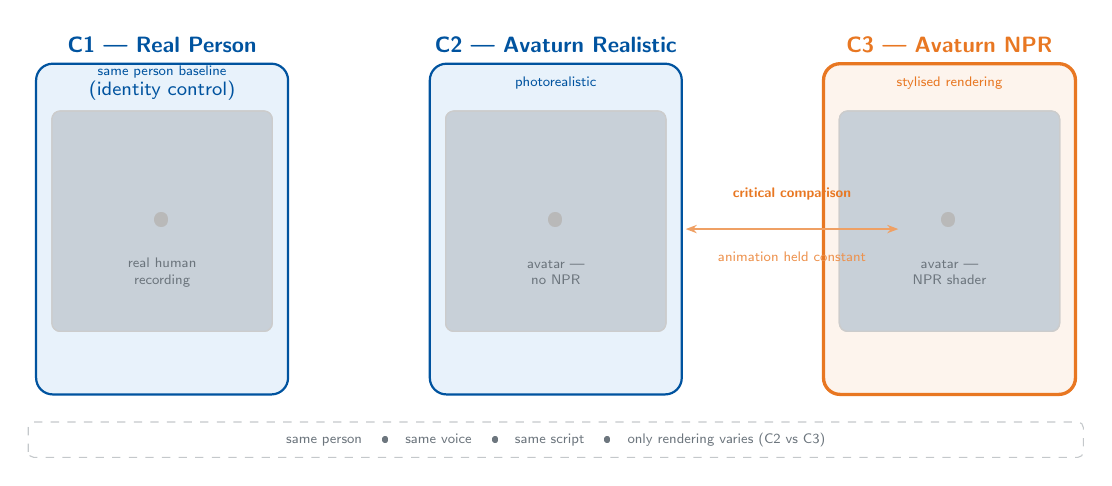
\begin{tikzpicture}[x=1cm, y=1cm]

  %% C1 — Real Person (centers raised to y=3.0 so boxes don't go off-slide)
  \node[condbox, label={[font=\footnotesize\sffamily\bfseries\color{kblue}]above:C1 — Real Person}]
    (c1) at (2.0,3.0) {};
  \fill[vidbox] (0.6,1.7) rectangle (3.4,4.5);
  \draw[gray!40, rounded corners=3pt] (0.6,1.7) rectangle (3.4,4.5);
  \node[font=\small\color{gray!55}] at (2.0,3.1) {\Large\textbullet};
  \node[font=\tiny\sffamily\color{kgray}, align=center] at (2.0,2.45) {real human\\ recording};
  \node[font=\tiny\sffamily\color{kblue}, align=center] at (2.0,4.85) {same person baseline\\{\scriptsize (identity control)}};

  %% C2 — Avaturn Realistic
  \node[condbox, label={[font=\footnotesize\sffamily\bfseries\color{kblue}]above:C2 — Avaturn Realistic}]
    (c2) at (7.0,3.0) {};
  \fill[vidbox] (5.6,1.7) rectangle (8.4,4.5);
  \draw[gray!40, rounded corners=3pt] (5.6,1.7) rectangle (8.4,4.5);
  \node[font=\small\color{gray!55}] at (7.0,3.1) {\Large\textbullet};
  \node[font=\tiny\sffamily\color{kgray}, align=center] at (7.0,2.45) {avatar ---\\ no NPR};
  \node[font=\tiny\sffamily\color{kblue}, align=center] at (7.0,4.85) {photorealistic};

  %% C3 — Avaturn NPR
  \node[condboxhi, label={[font=\footnotesize\sffamily\bfseries\color{korange}]above:C3 — Avaturn NPR}]
    (c3) at (12.0,3.0) {};
  \fill[vidbox] (10.6,1.7) rectangle (13.4,4.5);
  \draw[gray!40, rounded corners=3pt] (10.6,1.7) rectangle (13.4,4.5);
  \node[font=\small\color{gray!55}] at (12.0,3.1) {\Large\textbullet};
  \node[font=\tiny\sffamily\color{kgray}, align=center] at (12.0,2.45) {avatar ---\\ NPR shader};
  \node[font=\tiny\sffamily\color{korange}, align=center] at (12.0,4.85) {stylised rendering};

  %% Shared constraint banner — clearly below the boxes (box bottom at y=0.9, banner at 0.1–0.52)
  \draw[kgray!40, dashed, rounded corners=2pt] (0.3,0.10) rectangle (13.7,0.55);
  \node[font=\tiny\sffamily\color{kgray}, align=center] at (7.0,0.32)
    {same person \quad\textbullet\quad same voice \quad\textbullet\quad
     same script \quad\textbullet\quad only rendering varies (C2 vs C3)};

  %% Critical comparison bracket
  \draw[korange!70, line width=1.0pt,
        {Stealth[length=4pt,width=3pt]}-{Stealth[length=4pt,width=3pt]}]
    (8.65,3.0) -- (11.35,3.0);
  \node[font=\tiny\sffamily\bfseries\color{korange}] at (10.0,3.45)
    {critical comparison};
  \node[font=\tiny\sffamily\color{korange!80}] at (10.0,2.65)
    {animation held constant};

\end{tikzpicture}
\end{center}
\end{frame}

%% ═══════════════════════════════════════════════════════════════════════════
%% SLIDE 2 — Three Scenarios Overview
%% ═══════════════════════════════════════════════════════════════════════════
%% ── Three Advisor Scenarios — horizontal-row layout ─────────────────────
%% Three rows, one per scenario. Columns: badge | context | opt-A | opt-B | recommends
\begin{frame}{Three Advisor Scenarios}
\begin{center}
\resizebox{0.97\textwidth}{!}{%
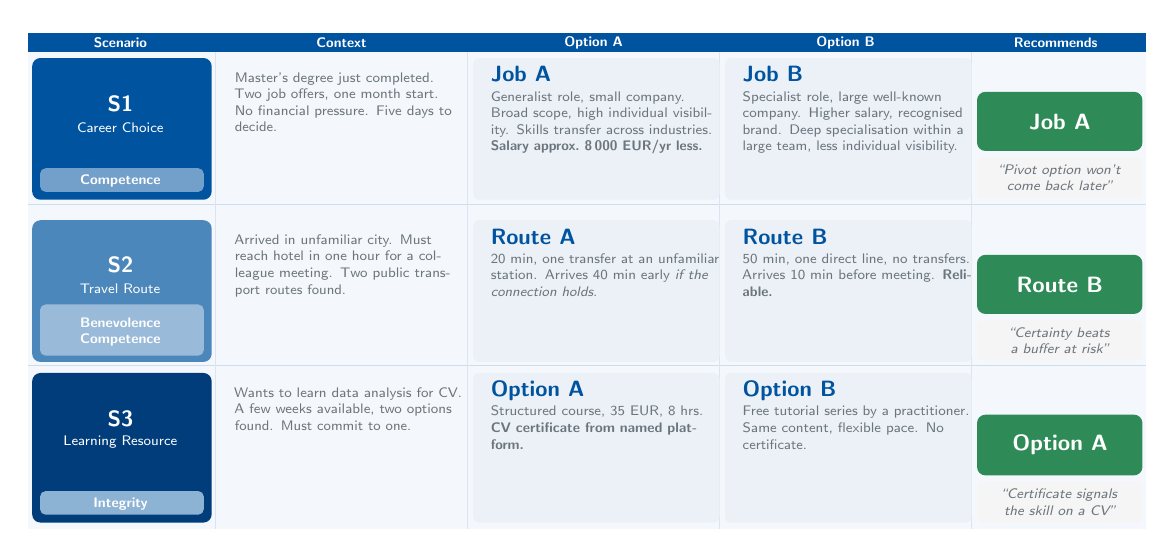
\begin{tikzpicture}[x=1cm, y=1cm]

%% Column x boundaries (total width ~14.2)
%% badge: 0.0 – 2.35
%% context: 2.45 – 5.55
%% opt-A: 5.65 – 8.85
%% opt-B: 8.95 – 12.15
%% rec: 12.25 – 14.2

%% Row y boundaries (each row height 1.95, gap 0.15)
%% Row 1 top: y=[4.25, 6.20]  Row 2: y=[2.15, 4.10]  Row 3: y=[0.05, 2.00]

%% ── helper fills for header + separator lines ─────────────────────────────
\fill[kbluepale] (0.0,0.0) rectangle (14.2,6.3);
%% Horizontal dividers
\draw[kblue!20, line width=0.4pt] (0.0,4.12) -- (14.2,4.12);
\draw[kblue!20, line width=0.4pt] (0.0,2.07) -- (14.2,2.07);
%% Vertical dividers
\foreach \x in {2.38, 5.58, 8.78, 11.98} {
  \draw[kblue!15, line width=0.3pt] (\x,0.0) -- (\x,6.3);
}

%% Column headers (top strip)
\fill[kblue] (0.0,6.05) rectangle (14.2,6.3);
\node[font=\tiny\sffamily\bfseries, text=white] at (1.17,6.17) {Scenario};
\node[font=\tiny\sffamily\bfseries, text=white] at (3.98,6.17) {Context};
\node[font=\tiny\sffamily\bfseries, text=white] at (7.18,6.17) {Option A};
\node[font=\tiny\sffamily\bfseries, text=white] at (10.38,6.17) {Option B};
\node[font=\tiny\sffamily\bfseries, text=white] at (13.05,6.17) {Recommends};

%% ══════════════════════════════════════════════════════════════════════════
%% ROW 1 — Scenario 1: Career Choice (y = 4.15 to 6.00)
%% ══════════════════════════════════════════════════════════════════════════
%% Badge cell
\fill[kblue, rounded corners=3pt] (0.05,4.18) rectangle (2.33,5.98);
\node[font=\footnotesize\sffamily\bfseries, text=white, align=center] at (1.17,5.40)
  {S1};
\node[font=\tiny\sffamily, text=white!85, align=center, text width=2.1cm] at (1.17,5.10)
  {Career Choice};
\fill[kblue!55, rounded corners=2pt] (0.15,4.28) rectangle (2.23,4.58);
\node[font=\tiny\sffamily\bfseries, text=white, align=center, text width=1.95cm]
  at (1.17,4.42) {Competence};

%% Context cell
\node[font=\tiny\sffamily\color{kgray}, text width=2.9cm, anchor=north west]
  at (2.50,5.92)
  {Master's degree just completed. Two job offers, one month start.
   No financial pressure. Five days to decide.};

%% Option A cell
\fill[kblue!8, rounded corners=2pt] (5.65,4.18) rectangle (8.78,5.98);
\node[font=\footnotesize\sffamily\bfseries\color{kblue}, anchor=north west] at (5.75,6)
  {Job A};
\node[font=\tiny\sffamily\color{kgray}, text width=2.9cm, anchor=north west] at (5.75,5.68)
  {Generalist role, small company. Broad scope, high individual visibility.
   Skills transfer across industries.
   \textbf{Salary approx.\ 8\,000 EUR/yr less.}};

%% Option B cell
\fill[kblue!8, rounded corners=2pt] (8.85,4.18) rectangle (11.98,5.98);
\node[font=\footnotesize\sffamily\bfseries\color{kblue}, anchor=north west] at (8.95,6)
  {Job B};
\node[font=\tiny\sffamily\color{kgray}, text width=2.9cm, anchor=north west] at (8.95,5.68)
  {Specialist role, large well-known company. Higher salary, recognised brand.
   Deep specialisation within a large team, less individual visibility.};

%% Recommends cell
\fill[kgreen, rounded corners=3pt] (12.05,4.80) rectangle (14.15,5.55);
\node[font=\footnotesize\sffamily\bfseries, text=white, align=center, text width=1.9cm]
  at (13.10,5.17) {Job A};
\fill[gray!8, rounded corners=2pt] (12.05,4.20) rectangle (14.15,4.72);
\node[font=\tiny\sffamily\itshape\color{kgray}, text width=1.9cm, align=center]
  at (13.10,4.46)
  {``Pivot option won't come back later''};

%% ══════════════════════════════════════════════════════════════════════════
%% ROW 2 — Scenario 2: Travel Route (y = 2.08 to 4.08)
%% ══════════════════════════════════════════════════════════════════════════
\fill[kblue!70, rounded corners=3pt] (0.05,2.12) rectangle (2.33,3.92);
\node[font=\footnotesize\sffamily\bfseries, text=white, align=center] at (1.17,3.35)
  {S2};
\node[font=\tiny\sffamily, text=white!85, align=center, text width=2.1cm] at (1.17,3.05)
  {Travel Route};
\fill[kblue!40, rounded corners=2pt] (0.15,2.2) rectangle (2.23,2.85);
\node[font=\tiny\sffamily\bfseries, text=white, align=center, text width=1.95cm]
  at (1.17,2.5) {Benevolence\\Competence};

\node[font=\tiny\sffamily\color{kgray}, text width=2.9cm, anchor=north west]
  at (2.50,3.86)
  {Arrived in unfamiliar city. Must reach hotel in one hour for a colleague meeting.
   Two public transport routes found.};

\fill[kblue!8, rounded corners=2pt] (5.65,2.12) rectangle (8.78,3.92);
\node[font=\footnotesize\sffamily\bfseries\color{kblue}, anchor=north west] at (5.75,3.93)
  {Route A};
\node[font=\tiny\sffamily\color{kgray}, text width=2.9cm, anchor=north west] at (5.75,3.62)
  {20 min, one transfer at an unfamiliar station.
   Arrives 40 min early \textit{if the connection holds.}};

\fill[kblue!8, rounded corners=2pt] (8.85,2.12) rectangle (11.98,3.92);
\node[font=\footnotesize\sffamily\bfseries\color{kblue}, anchor=north west] at (8.95,3.93)
  {Route B};
\node[font=\tiny\sffamily\color{kgray}, text width=2.9cm, anchor=north west] at (8.95,3.62)
  {50 min, one direct line, no transfers.
   Arrives 10 min before meeting. \textbf{Reliable.}};

\fill[kgreen, rounded corners=3pt] (12.05,2.73) rectangle (14.15,3.48);
\node[font=\footnotesize\sffamily\bfseries, text=white, align=center, text width=1.9cm]
  at (13.10,3.10) {Route B};
\fill[gray!8, rounded corners=2pt] (12.05,2.14) rectangle (14.15,2.65);
\node[font=\tiny\sffamily\itshape\color{kgray}, text width=1.9cm, align=center]
  at (13.10,2.39)
  {``Certainty beats a buffer at risk''};

%% ══════════════════════════════════════════════════════════════════════════
%% ROW 3 — Scenario 3: Learning Resource (y = 0.05 to 2.02)
%% ══════════════════════════════════════════════════════════════════════════
\fill[kbluedark, rounded corners=3pt] (0.05,0.08) rectangle (2.33,1.98);
\node[font=\footnotesize\sffamily\bfseries, text=white, align=center] at (1.17,1.40)
  {S3};
\node[font=\tiny\sffamily, text=white!85, align=center, text width=2.1cm] at (1.17,1.10)
  {Learning Resource};
\fill[kblue!45, rounded corners=2pt] (0.15,0.18) rectangle (2.23,0.48);
\node[font=\tiny\sffamily\bfseries, text=white, align=center, text width=1.95cm]
  at (1.17,0.32) {Integrity};

\node[font=\tiny\sffamily\color{kgray}, text width=2.9cm, anchor=north west]
  at (2.50,1.92)
  {Wants to learn data analysis for CV. A few weeks available, two options found.
   Must commit to one.};

\fill[kblue!8, rounded corners=2pt] (5.65,0.08) rectangle (8.78,1.98);
\node[font=\footnotesize\sffamily\bfseries\color{kblue}, anchor=north west] at (5.75,2)
  {Option A};
\node[font=\tiny\sffamily\color{kgray}, text width=2.9cm, anchor=north west] at (5.75,1.68)
  {Structured course, 35 EUR, 8 hrs.
   \textbf{CV certificate from named platform.}};

\fill[kblue!8, rounded corners=2pt] (8.85,0.08) rectangle (11.98,1.98);
\node[font=\footnotesize\sffamily\bfseries\color{kblue}, anchor=north west] at (8.95,2)
  {Option B};
\node[font=\tiny\sffamily\color{kgray}, text width=2.9cm, anchor=north west] at (8.95,1.68)
  {Free tutorial series by a practitioner. Same content, flexible pace.
   No certificate.};

\fill[kgreen, rounded corners=3pt] (12.05,0.68) rectangle (14.15,1.45);
\node[font=\footnotesize\sffamily\bfseries, text=white, align=center, text width=1.9cm]
  at (13.10,1.07) {Option A};
\fill[gray!8, rounded corners=2pt] (12.05,0.08) rectangle (14.15,0.60);
\node[font=\tiny\sffamily\itshape\color{kgray}, text width=1.9cm, align=center]
  at (13.10,0.34)
  {``Certificate signals the skill on a CV''};

\end{tikzpicture}%
}
\end{center}
\end{frame}

%% ═══════════════════════════════════════════════════════════════════════════
%% SLIDE 2b — What the Avatar Says (Recommendation Scripts)
%% ═══════════════════════════════════════════════════════════════════════════
\begin{frame}{What the Avatar Says — Recommendation Scripts}
\begin{center}
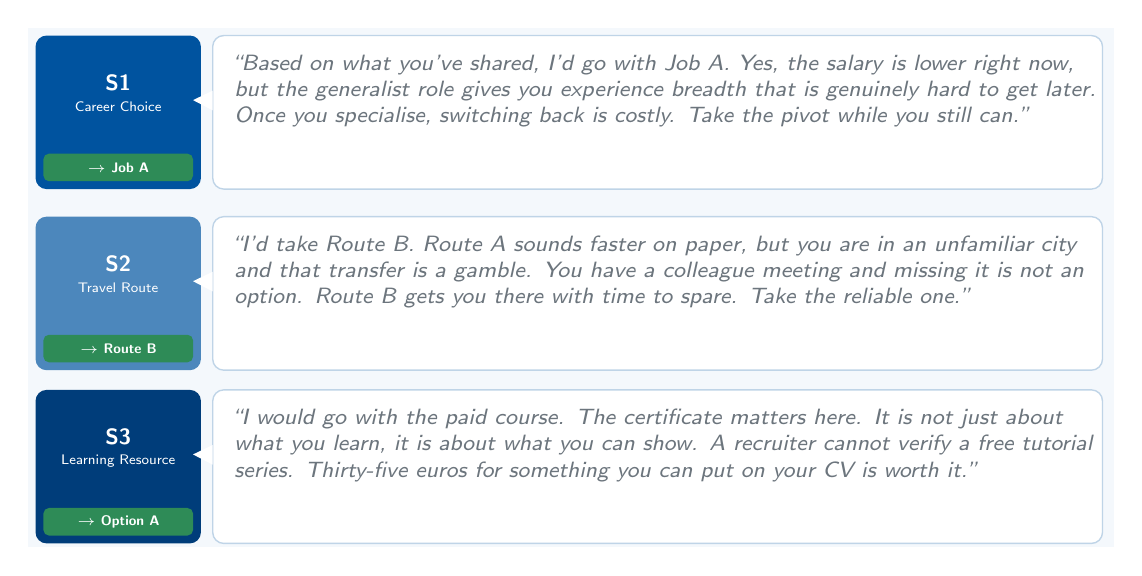
\begin{tikzpicture}[x=1cm, y=1cm]

%% Background
\fill[kbluepale] (0.0,0.0) rectangle (13.8,6.6);

%% ── S1 Career Choice ────────────────────────────────────────────────────
\fill[kblue, rounded corners=4pt] (0.1,4.55) rectangle (2.20,6.50);
\node[font=\footnotesize\sffamily\bfseries, text=white, align=center] at (1.15,5.90) {S1};
\node[font=\tiny\sffamily, text=white!85, align=center, text width=1.95cm] at (1.15,5.60) {Career Choice};
\fill[kgreen, rounded corners=2pt] (0.20,4.65) rectangle (2.10,5.00);
\node[font=\tiny\sffamily\bfseries, text=white, align=center] at (1.15,4.82) {$\rightarrow$ Job A};

%% Speech bubble S1
\fill[white, rounded corners=4pt] (2.35,4.55) rectangle (13.65,6.50);
\draw[kblue!25, rounded corners=4pt, line width=0.5pt] (2.35,4.55) rectangle (13.65,6.50);
%% triangle pointer
\fill[white] (2.35,5.80) -- (2.10,5.68) -- (2.35,5.55) -- cycle;
\node[font=\footnotesize\sffamily\itshape\color{kgray}, text width=10.9cm, anchor=north west]
  at (2.50,6.38)
  {``Based on what you've shared, I'd go with Job A. Yes, the salary is lower right now, but the generalist role gives you experience breadth that is genuinely hard to get later. Once you specialise, switching back is costly. Take the pivot while you still can.''};

%% ── S2 Travel Route ─────────────────────────────────────────────────────
\fill[kblue!70, rounded corners=4pt] (0.1,2.25) rectangle (2.20,4.20);
\node[font=\footnotesize\sffamily\bfseries, text=white, align=center] at (1.15,3.60) {S2};
\node[font=\tiny\sffamily, text=white!85, align=center, text width=1.95cm] at (1.15,3.30) {Travel Route};
\fill[kgreen, rounded corners=2pt] (0.20,2.35) rectangle (2.10,2.70);
\node[font=\tiny\sffamily\bfseries, text=white, align=center] at (1.15,2.52) {$\rightarrow$ Route B};

%% Speech bubble S2
\fill[white, rounded corners=4pt] (2.35,2.25) rectangle (13.65,4.20);
\draw[kblue!25, rounded corners=4pt, line width=0.5pt] (2.35,2.25) rectangle (13.65,4.20);
\fill[white] (2.35,3.50) -- (2.10,3.38) -- (2.35,3.25) -- cycle;
\node[font=\footnotesize\sffamily\itshape\color{kgray}, text width=10.9cm, anchor=north west]
  at (2.50,4.08)
  {``I'd take Route B. Route A sounds faster on paper, but you are in an unfamiliar city and that transfer is a gamble. You have a colleague meeting and missing it is not an option. Route B gets you there with time to spare. Take the reliable one.''};

%% ── S3 Learning Resource ────────────────────────────────────────────────
\fill[kbluedark, rounded corners=4pt] (0.1,0.05) rectangle (2.20,2.00);
\node[font=\footnotesize\sffamily\bfseries, text=white, align=center] at (1.15,1.40) {S3};
\node[font=\tiny\sffamily, text=white!85, align=center, text width=1.95cm] at (1.15,1.10) {Learning Resource};
\fill[kgreen, rounded corners=2pt] (0.20,0.15) rectangle (2.10,0.50);
\node[font=\tiny\sffamily\bfseries, text=white, align=center] at (1.15,0.32) {$\rightarrow$ Option A};

%% Speech bubble S3
\fill[white, rounded corners=4pt] (2.35,0.05) rectangle (13.65,2.00);
\draw[kblue!25, rounded corners=4pt, line width=0.5pt] (2.35,0.05) rectangle (13.65,2.00);
\fill[white] (2.35,1.30) -- (2.10,1.18) -- (2.35,1.05) -- cycle;
\node[font=\footnotesize\sffamily\itshape\color{kgray}, text width=10.9cm, anchor=north west]
  at (2.50,1.88)
  {``I would go with the paid course. The certificate matters here. It is not just about what you learn, it is about what you can show. A recruiter cannot verify a free tutorial series. Thirty-five euros for something you can put on your CV is worth it.''};

\end{tikzpicture}
\end{center}
\end{frame}


%% ═══════════════════════════════════════════════════════════════════════════
%% SLIDE — Video Production Checklist (researcher note)
%% ═══════════════════════════════════════════════════════════════════════════
\begin{frame}{Video Production Checklist \textnormal{\small (researcher note — before recording)}}
\small
\begin{columns}[T]
\begin{column}{0.48\textwidth}
\textbf{\color{kblue}Match across C1, C2, C3}
\begin{itemize}\setlength\itemsep{3pt}
  \item \textbf{Resolution \& ratio:} 1920$\times$1080, 16:9 for all three
  \item \textbf{Frame rate:} 30 fps — Unity export must match camera
  \item \textbf{Duration:} within $\pm$1 s per scenario
  \item \textbf{Framing:} eye-level, centred, same head-to-shoulder crop
  \item \textbf{Background:} same desk, setting, camera angle replicated in Unity scene
\end{itemize}
\end{column}
\begin{column}{0.48\textwidth}
\textbf{\color{kblue}Audio \& technical}
\begin{itemize}\setlength\itemsep{3pt}
  \item \textbf{Audio:} one recording, same mic and room, applied to all three; normalise to $-16$ LUFS
  \item \textbf{No TTS} in any condition
  \item \textbf{Lighting colour:} match Unity light temperature to C1 camera environment
  \item \textbf{Codec:} H.264 MP4, same bitrate for all three
\end{itemize}
\vspace{6pt}
% \begin{alertblock}{\small Pilot check}
% \small Watch all three side by side. If you can identify C1 by \textit{production quality alone} (not avatar appearance), adjust before data collection.
% \end{alertblock}
\end{column}
\end{columns}
\end{frame}

%% ═══════════════════════════════════════════════════════════════════════════
%% SLIDE 4 — Full Study Flow Overview
%% ═══════════════════════════════════════════════════════════════════════════
\begin{frame}{Study Flow Overview}
\begin{center}
\resizebox{0.96\textwidth}{!}{%
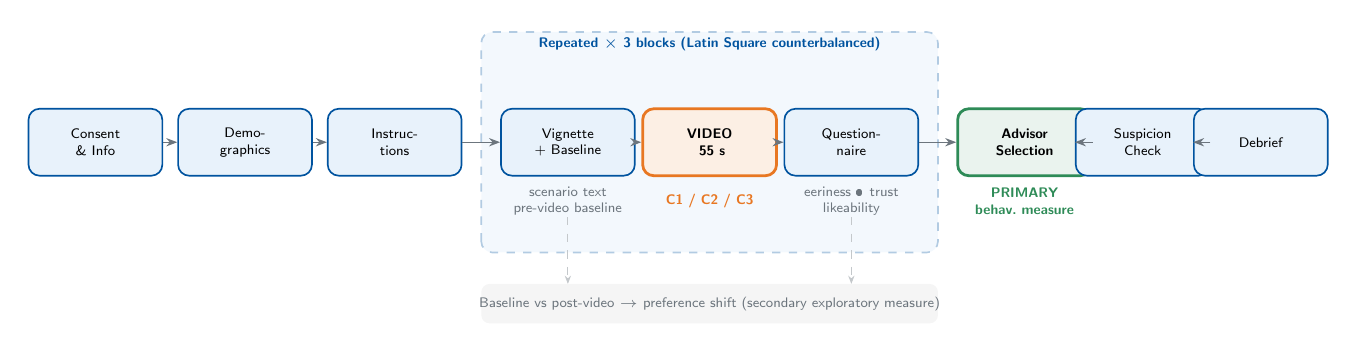
\begin{tikzpicture}[x=1cm, y=1cm]

  \node[fbox] (consent) at (0.9,4.2) {Consent\\\& Info};
  \node[fbox] (demo)    at (2.8,4.2) {Demo-\\graphics};
  \node[fbox] (inst)    at (4.7,4.2) {Instruc-\\tions};

  %% Repeated block bracket
  \fill[kbluelight!50, rounded corners=4pt] (5.8,2.8) rectangle (11.6,5.6);
  \draw[kblue!30, rounded corners=4pt, dashed, line width=0.6pt] (5.8,2.8) rectangle (11.6,5.6);
  \node[font=\tiny\sffamily\bfseries\color{kblue}] at (8.7,5.45)
    {Repeated $\times$ 3 blocks (Latin Square counterbalanced)};

  \node[fbox]     (vign)   at (6.9,4.2) {Vignette\\ + Baseline};
  \node[fboxhi]   (vid)    at (8.7,4.2) {VIDEO\\ \textbf{$\blacktriangleright$\ 55 s}};
  \node[fbox]     (scales) at (10.5,4.2) {Question-\\naire};

  \node[fboxgreen] (post)    at (12.7,4.2) {Advisor\\Selection};
  \node[fbox]      (funnel)  at (14.2,4.2) {Suspicion\\Check};
  \node[fbox]      (debrief) at (15.7,4.2) {Debrief};

  %% Arrows
  \foreach \a/\b in {consent/demo, demo/inst, inst/vign, vign/vid, vid/scales} {
    \draw[farrow] (\a) -- (\b);
  }
  \draw[farrow] (scales.east) -- (post.west);
  \foreach \a/\b in {post/funnel, funnel/debrief} {
    \draw[farrow] (\a) -- (\b);
  }

  %% Sub-labels
  \node[font=\tiny\color{kgray}, align=center] at (6.9,3.45)
    {scenario text\\ pre-video baseline};
  \node[font=\tiny\color{korange}\bfseries, align=center] at (8.7,3.45)
    {C1 / C2 / C3};
  \node[font=\tiny\color{kgray}, align=center] at (10.5,3.45)
    {eeriness \textbullet\ trust\\ likeability};
  \node[font=\tiny\color{kgreen}\bfseries, align=center] at (12.7,3.45)
    {PRIMARY\\behav.\ measure};

  %% Secondary measure note
  \draw[kgray!40, -{Stealth[length=3pt]}, dashed] (6.9,3.25) -- (6.9,2.4);
  \draw[kgray!40, -{Stealth[length=3pt]}, dashed] (10.5,3.25) -- (10.5,2.4);
  \fill[gray!8, rounded corners=3pt] (5.8,1.9) rectangle (11.6,2.4);
  \node[font=\tiny\sffamily\color{kgray}, align=center] at (8.7,2.15)
    {Baseline vs post-video $\to$ preference shift (secondary exploratory measure)};

\end{tikzpicture}%
}
\end{center}
\end{frame}

%% ═══════════════════════════════════════════════════════════════════════════
%% SLIDE 12 — Scene 1: Welcome / Consent
%% ═══════════════════════════════════════════════════════════════════════════
\begin{frame}{Scene 1 — Welcome \& Consent}
\begin{center}
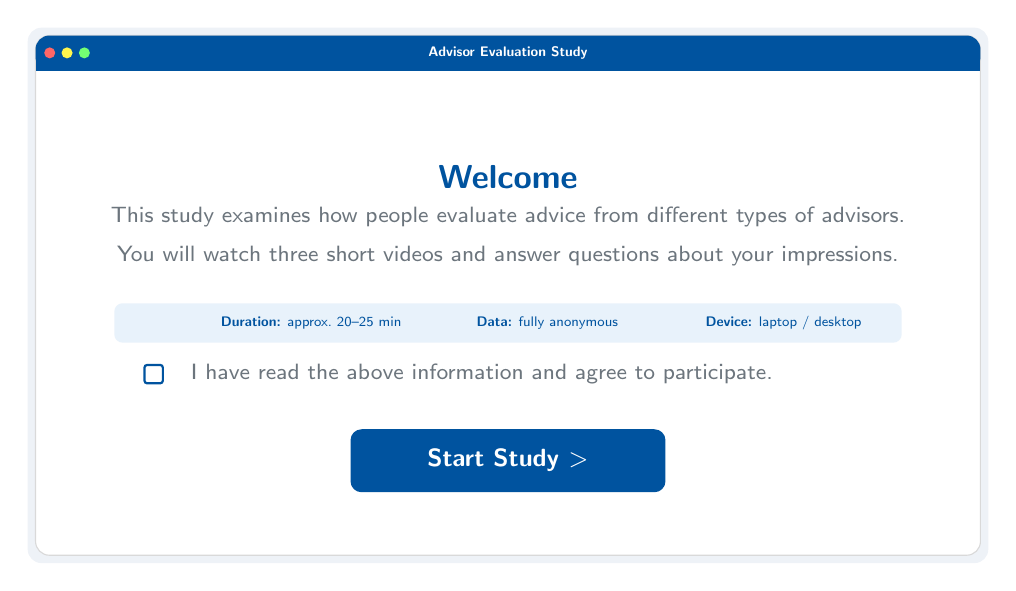
\begin{tikzpicture}[x=1cm, y=1cm]

  \browserchrome{1.0}{0.2}{13.0}{6.8}{Advisor Evaluation Study}
  %\progressbar{1.5}{6.2}{12.5}{0.13}{Step 1 of 8}

  \node[font=\large\sffamily\bfseries\color{kblue}] at (7.0,5) {Welcome};

  \node[font=\footnotesize\sffamily\color{kgray}, align=center]
    at (7.0,4.5) {This study examines how people evaluate advice from different types of advisors.};
  \node[font=\footnotesize\sffamily\color{kgray}, align=center]
    at (7.0,4) {You will watch three short videos and answer questions about your impressions.};

  \fill[kbluelight, rounded corners=3pt] (2.0,3.4) rectangle (12.0,2.9);
  \node[font=\tiny\sffamily\color{kblue}] at (4.5,3.15) {\textbf{Duration:} approx.\ 20--25 min};
  \node[font=\tiny\sffamily\color{kblue}] at (7.5,3.15) {\textbf{Data:} fully anonymous};
  \node[font=\tiny\sffamily\color{kblue}] at (10.5,3.15) {\textbf{Device:} laptop / desktop};

  \node[checkbox] (cb) at (2.5,2.5) {};
  \node[font=\footnotesize\sffamily\color{kgray}, anchor=west] at (2.85,2.5)
    {I have read the above information and agree to participate.};

  \fill[kblue, rounded corners=4pt] (5.0,1) rectangle (9.0,1.8);
  \node[font=\small\sffamily\bfseries, text=white] at (7.0,1.4) {Start Study \textbf{\textgreater}};

\end{tikzpicture}
\end{center}
\end{frame}

%% ═══════════════════════════════════════════════════════════════════════════
%% SLIDE 13 — Scene 2: Participant Instruction
%% ═══════════════════════════════════════════════════════════════════════════
\begin{frame}{Scene 2 — Participant Instruction}
\begin{center}
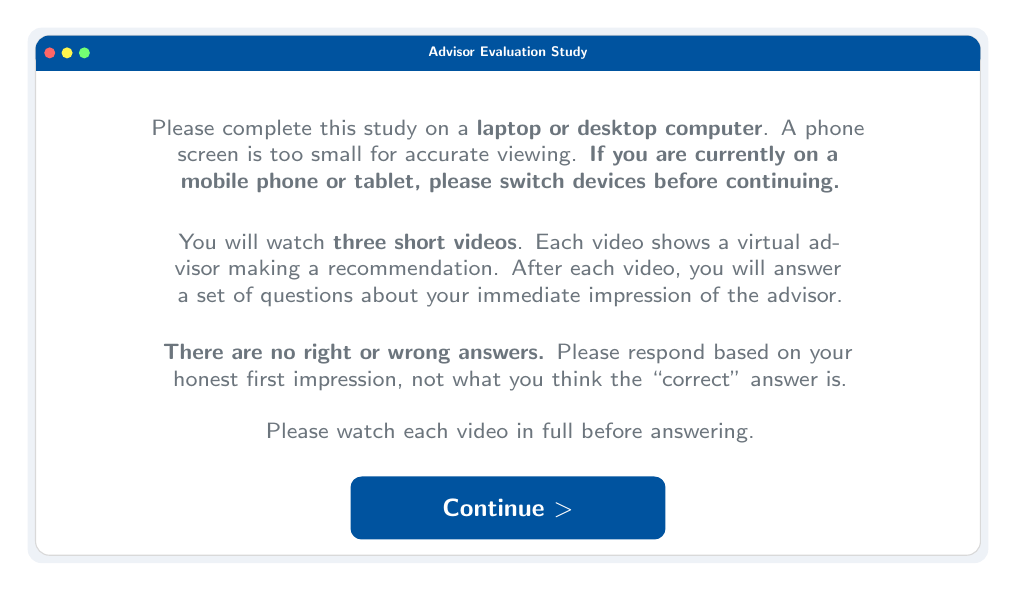
\begin{tikzpicture}[x=1cm, y=1cm]

  \browserchrome{1.0}{0.2}{13.0}{6.8}{Advisor Evaluation Study}
  %\progressbar{1.5}{6.2}{12.5}{0.23}{Step 2 of 8}

  % \node[font=\large\sffamily\bfseries\color{kblue}] at (7.0,5) {Welcome};

  \node[font=\footnotesize\sffamily\color{kgray}, text width=11.0cm, align=center, anchor=north]
    at (7.0,5.85) {Please complete this study on a \textbf{laptop or desktop computer}. A phone screen is too small for accurate viewing. \textbf{If you are currently on a mobile phone or tablet, please switch devices before continuing.}};

  \node[font=\footnotesize\sffamily\color{kgray}, text width=11.0cm, align=center, anchor=north]
    at (7.0,4.4) {You will watch \textbf{three short videos}. Each video shows a virtual advisor making a recommendation. After each video, you will answer a set of questions about your immediate impression of the advisor.};

  \node[font=\footnotesize\sffamily\color{kgray}, text width=11.0cm, align=center, anchor=north]
    at (7.0,3) {\textbf{There are no right or wrong answers.} Please respond based on your honest first impression, not what you think the ``correct'' answer is.};

  \node[font=\footnotesize\sffamily\color{kgray}, text width=11.0cm, align=center, anchor=north]
    at (7.0,2) {Please watch each video in full before answering.};

  % \fill[kbluelight, rounded corners=3pt] (2.0,3.4) rectangle (12.0,2.9);
  % \node[font=\tiny\sffamily\color{kblue}] at (4.5,3.15) {\textbf{Duration:} approx.\ 20--25 min};
  % \node[font=\tiny\sffamily\color{kblue}] at (7.5,3.15) {\textbf{Data:} fully anonymous};
  % \node[font=\tiny\sffamily\color{kblue}] at (10.5,3.15) {\textbf{Device:} laptop / desktop};

  % \node[checkbox] (cb) at (2.5,2.5) {};
  % \node[font=\footnotesize\sffamily\color{kgray}, anchor=west] at (2.85,2.5)
  %   {I have read the above information and agree to participate.};

  \fill[kblue, rounded corners=4pt] (5.0,0.4) rectangle (9.0,1.2);
  \node[font=\small\sffamily\bfseries, text=white] at (7.0,0.8) {Continue \textbf{\textgreater}};

\end{tikzpicture}
\end{center}
\end{frame}


%% ═══════════════════════════════════════════════════════════════════════════
%% DEMOGRAPHICS 1/2 — Basic Information
%% ═══════════════════════════════════════════════════════════════════════════
\begin{frame}{Scene 2b — Demographics (1 of 2)}
\begin{center}
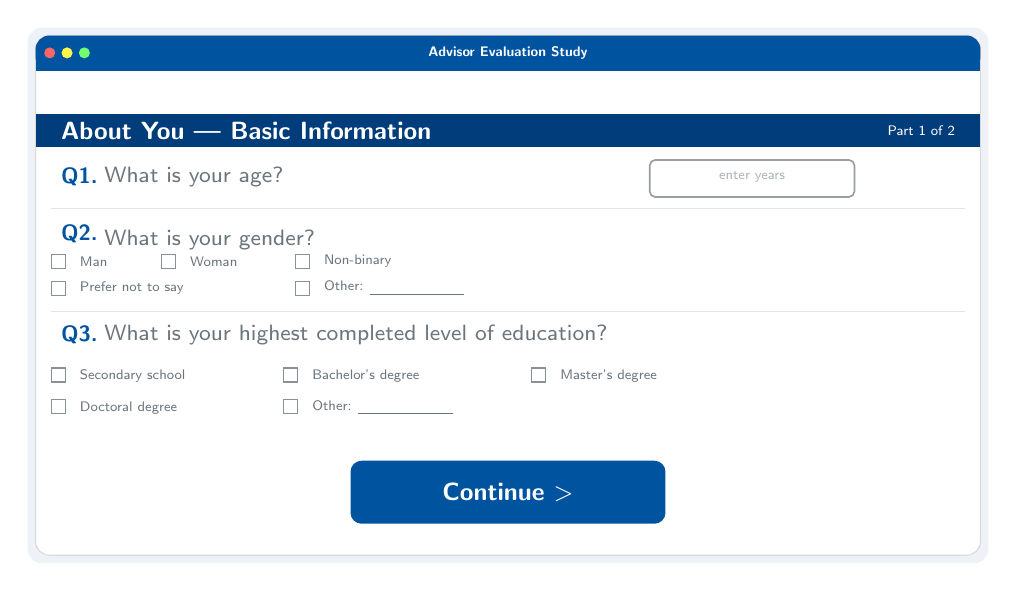
\begin{tikzpicture}[x=1cm, y=1cm]

  \browserchrome{1.0}{0.2}{13.0}{6.8}{Advisor Evaluation Study}
  %\progressbar{1.5}{6.20}{12.5}{0.30}{Step 3 of 9}

  %% Section header
  \fill[kbluedark] (1.0,5.38) rectangle (13.0,5.80);
  \node[font=\small\sffamily\bfseries, text=white, anchor=west] at (1.20,5.59)
    {About You --- Basic Information};
  \node[font=\tiny\sffamily, text=white!75, anchor=east] at (12.80,5.59)
    {Part 1 of 2};

  %% Q1: Age
  \node[font=\footnotesize\sffamily\bfseries\color{kblue}, anchor=west] at (1.20,5.)
    {Q1.};
  \node[font=\footnotesize\sffamily\color{kgray}, anchor=west] at (1.75,5)
    {What is your age?};
  \draw[kgray!70, rounded corners=2pt, line width=0.6pt]
    (8.80,4.75) rectangle (11.40,5.22);
  \node[font=\tiny\sffamily\color{kgray!55}] at (10.10,5) {enter years};

  \draw[kgray!20, line width=0.4pt] (1.20,4.6) -- (12.80,4.6);

  %% Q2: Gender
  \node[font=\footnotesize\sffamily\bfseries\color{kblue}, anchor=west] at (1.20,4.28)
    {Q2.};
  \node[font=\footnotesize\sffamily\color{kgray}, anchor=west] at (1.75,4.20)
    {What is your gender?};
  \draw[kgray!80, line width=0.5pt] (1.20,3.84) rectangle (1.38,4.02);
  \node[font=\tiny\sffamily\color{kgray}, anchor=west] at (1.44,3.93) {Man};
  \draw[kgray!80, line width=0.5pt] (2.60,3.84) rectangle (2.78,4.02);
  \node[font=\tiny\sffamily\color{kgray}, anchor=west] at (2.84,3.93) {Woman};
  \draw[kgray!80, line width=0.5pt] (4.30,3.84) rectangle (4.48,4.02);
  \node[font=\tiny\sffamily\color{kgray}, anchor=west] at (4.54,3.93) {Non-binary};
  \draw[kgray!80, line width=0.5pt] (1.20,3.68) rectangle (1.38,3.5);
  \node[font=\tiny\sffamily\color{kgray}, anchor=west] at (1.44,3.59) {Prefer not to say};
  \draw[kgray!80, line width=0.5pt] (4.30,3.68) rectangle (4.48,3.5);
  \node[font=\tiny\sffamily\color{kgray}, anchor=west] at (4.54,3.59) {Other: \underline{\hspace{1.2cm}}};

  \draw[kgray!20, line width=0.4pt] (1.20,3.3) -- (12.80,3.3);

  %% Q3: Education
  \node[font=\footnotesize\sffamily\bfseries\color{kblue}, anchor=west] at (1.20,3.)
    {Q3.};
  \node[font=\footnotesize\sffamily\color{kgray}, anchor=west] at (1.75,3)
    {What is your highest completed level of education?};
  \draw[kgray!80, line width=0.5pt] (1.20,2.58) rectangle (1.38,2.4);
  \node[font=\tiny\sffamily\color{kgray}, anchor=west] at (1.44,2.47) {Secondary school};
  \draw[kgray!80, line width=0.5pt] (4.15,2.58) rectangle (4.33,2.4);
  \node[font=\tiny\sffamily\color{kgray}, anchor=west] at (4.39,2.47) {Bachelor's degree};
  \draw[kgray!80, line width=0.5pt] (7.30,2.58) rectangle (7.48,2.4);
  \node[font=\tiny\sffamily\color{kgray}, anchor=west] at (7.54,2.47) {Master's degree};
  \draw[kgray!80, line width=0.5pt] (1.20,2.18) rectangle (1.38,2.);
  \node[font=\tiny\sffamily\color{kgray}, anchor=west] at (1.44,2.07) {Doctoral degree};
  \draw[kgray!80, line width=0.5pt] (4.15,2.18) rectangle (4.33,2);
  \node[font=\tiny\sffamily\color{kgray}, anchor=west] at (4.39,2.07) {Other: \underline{\hspace{1.2cm}}};

  \fill[kblue, rounded corners=4pt] (5.0,0.60) rectangle (9.0,1.40);
  \node[font=\small\sffamily\bfseries, text=white] at (7.0,1.0)
    {Continue \textbf{\textgreater}};

\end{tikzpicture}
\end{center}
\end{frame}

%% ═══════════════════════════════════════════════════════════════════════════
%% DEMOGRAPHICS 2/2 — Avatar Experience & Trust Baseline
%% ═══════════════════════════════════════════════════════════════════════════
\begin{frame}{Scene 2c — Demographics (2 of 2)}
\begin{center}
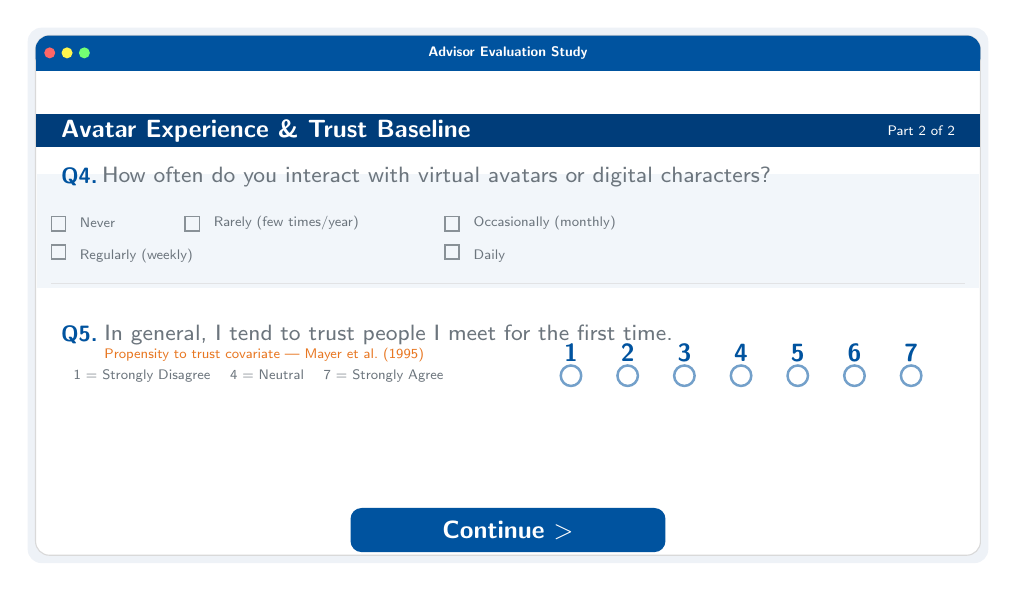
\begin{tikzpicture}[x=1cm, y=1cm]

  \browserchrome{1.0}{0.2}{13.0}{6.8}{Advisor Evaluation Study}
  %\progressbar{1.5}{6.20}{12.5}{0.40}{Step 4 of 9}

  %% Section header
  \fill[kbluedark] (1.0,5.38) rectangle (13.0,5.80);
  \node[font=\small\sffamily\bfseries, text=white, anchor=west] at (1.20,5.59)
    {Avatar Experience \& Trust Baseline};
  \node[font=\tiny\sffamily, text=white!75, anchor=east] at (12.80,5.59)
    {Part 2 of 2};

  %% Q4: Avatar usage
  \fill[kblue!5] (1.02,3.6) rectangle (12.98,5.04);
  \node[font=\footnotesize\sffamily\bfseries\color{kblue}, anchor=west] at (1.20,5.)
    {Q4.};
  \node[font=\footnotesize\sffamily\color{kgray}, anchor=west] at (1.72,5)
    {How often do you interact with virtual avatars or digital characters?};
  \draw[kgray!80, line width=0.5pt] (1.20,4.32) rectangle (1.38,4.50);
  \node[font=\tiny\sffamily\color{kgray}, anchor=west] at (1.44,4.42) {Never};
  \draw[kgray!80, line width=0.5pt] (2.90,4.32) rectangle (3.08,4.50);
  \node[font=\tiny\sffamily\color{kgray}, anchor=west] at (3.14,4.42) {Rarely (few times/year)};
  \draw[kgray!80, line width=0.5pt] (6.20,4.32) rectangle (6.38,4.50);
  \node[font=\tiny\sffamily\color{kgray}, anchor=west] at (6.44,4.42) {Occasionally (monthly)};
  \draw[kgray!80, line width=0.5pt] (1.20,3.96) rectangle (1.38,4.14);
  \node[font=\tiny\sffamily\color{kgray}, anchor=west] at (1.44,4) {Regularly (weekly)};
  \draw[kgray!80, line width=0.5pt] (6.20,3.96) rectangle (6.38,4.14);
  \node[font=\tiny\sffamily\color{kgray}, anchor=west] at (6.44,4) {Daily};

  \draw[kgray!20, line width=0.4pt] (1.20,3.65) -- (12.80,3.65);

  %% Q5 (formerly Q9): Propensity to trust — Mayer et al. (1995) covariate
  \node[font=\footnotesize\sffamily\bfseries\color{kblue}, anchor=west] at (1.20,3)
    {Q5.};
  \node[font=\footnotesize\sffamily\color{kgray}, anchor=west] at (1.75,3)
    {In general, I tend to trust people I meet for the first time.};
  \node[font=\tiny\sffamily\color{korange}, anchor=west] at (1.75,2.74)
    {Propensity to trust covariate --- Mayer et al.\ (1995)};

  \node[font=\tiny\sffamily\color{kgray}, anchor=west] at (1.36,2.47)
    {1 = Strongly Disagree \quad 4 = Neutral \quad 7 = Strongly Agree};
  \foreach \i/\n in {0/1,1/2,2/3,3/4,4/5,5/6,6/7}{
    \node[font=\small\sffamily\bfseries\color{kblue}] at ({7.8+\i*0.72},2.77) {\n};
  }
  \foreach \i in {0,1,2,3,4,5,6}{
    \draw[kblue!55, line width=0.9pt] ({7.8+\i*0.72},2.48) circle (0.13);
  }

  \fill[kblue, rounded corners=4pt] (5.0,0.24) rectangle (9.0,0.80);
  \node[font=\small\sffamily\bfseries, text=white] at (7.0,0.52)
    {Continue \textbf{\textgreater}};

\end{tikzpicture}
\end{center}
\end{frame}


%% ═══════════════════════════════════════════════════════════════════════════
%% SLIDE 3 — Scenario Detail: Scrolled Page View
%% ═══════════════════════════════════════════════════════════════════════════
\begin{frame}{Scene 3 — Scenario Page (Career Choice)}
\begin{center}
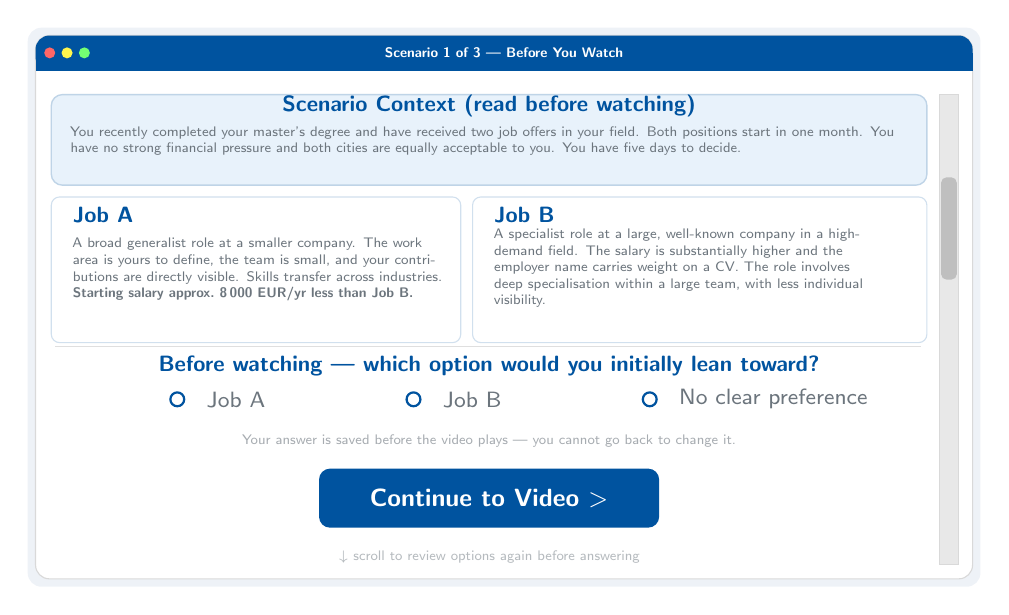
\begin{tikzpicture}[x=1cm, y=1cm]

  %% Browser window
  \browserchrome{0.4}{0.0}{12.3}{6.9}{Scenario 1 of 3 --- Before You Watch}

  %% Progress bar
  %\progressbar{0.9}{6.38}{11.8}{0.38}{Step 3 of 8}

  %% ── Scrollbar ──────────────────────────────────────────────────────────
  \fill[gray!18] (11.88,0.18) rectangle (12.12,6.15);
  \draw[gray!30, line width=0.3pt] (11.88,0.18) rectangle (12.12,6.15);
  %% Scroll thumb (positioned ~35% down, indicating content above)
  \fill[gray!50, rounded corners=2pt] (11.90,3.80) rectangle (12.10,5.10);
  %% Up/down arrow hints
  \node[font=\tiny\color{gray!55}] at (12.0,6.05) {$\scriptstyle\blacktriangle$};
  \node[font=\tiny\color{gray!55}] at (12.0,0.28) {$\scriptstyle\blacktriangledown$};

  %% ── Scenario header box (taller: bottom moved from 5.38 to 5.00) ──────
  \fill[kbluelight, draw=kblue!25, rounded corners=4pt, line width=0.5pt]
    (0.60,5.00) rectangle (11.72,6.15);
  \node[font=\footnotesize\sffamily\bfseries\color{kblue}] at (6.16,6.0)
    {Scenario Context (read before watching)};
  \node[font=\tiny\sffamily\color{kgray}, text width=10.5cm, anchor=north west]
    at (0.72,5.87)
    {You recently completed your master's degree and have received two job offers in your
     field. Both positions start in one month. You have no strong financial pressure and
     both cities are equally acceptable to you. You have five days to decide.};

  %% ── Option boxes (top lowered to 4.85, bottom to 3.55; titles reduced to \footnotesize) ─
  %% Option A
  \fill[white, draw=kblue!18, rounded corners=3pt, line width=0.4pt]
    (0.60,3) rectangle (5.80,4.85);
  \node[font=\footnotesize\sffamily\bfseries\color{kblue}, anchor=north west] at (0.75,4.85)
    {Job A};
  \node[font=\tiny\sffamily\color{kgray}, text width=4.7cm, anchor=north west]
    at (0.75,4.45)
    {A broad generalist role at a smaller company. The work area is yours to define,
     the team is small, and your contributions are directly visible.
     Skills transfer across industries.
     \textbf{Starting salary approx.\ 8\,000 EUR/yr less than Job B.}};

  %% Option B
  \fill[white, draw=kblue!18, rounded corners=3pt, line width=0.4pt]
    (5.95,3) rectangle (11.72,4.85);
  \node[font=\footnotesize\sffamily\bfseries\color{kblue}, anchor=north west] at (6.10,4.85)
    {Job B};
  \node[font=\tiny\sffamily\color{kgray}, text width=4.7cm, anchor=north west]
    at (6.10,4.57)
    {A specialist role at a large, well-known company in a high-demand field.
     The salary is substantially higher and the employer name carries weight on a CV.
     The role involves deep specialisation within a large team,
     with less individual visibility.};

  %% Divider
  \draw[gray!25, line width=0.3pt] (0.65,2.95) -- (11.65,2.95);

  %% Baseline question
  \node[font=\footnotesize\sffamily\bfseries\color{kblue}] at (6.16,2.7)
    {Before watching --- which option would you initially lean toward?};

  %% Radio options
  \node[radio] at (2.2,2.28) {};
  \node[font=\footnotesize\sffamily\color{kgray}, anchor=west] at (2.45,2.28) {Job A};
  \node[radio] at (5.2,2.28) {};
  \node[font=\footnotesize\sffamily\color{kgray}, anchor=west] at (5.45,2.28) {Job B};
  \node[radio] at (8.2,2.28) {};
  \node[font=\footnotesize\sffamily\color{kgray}, anchor=west] at (8.45,2.28)
    {No clear preference};

  %% Lock note
  \node[font=\tiny\sffamily\color{kgray!60}] at (6.16,1.75)
    {Your answer is saved before the video plays --- you cannot go back to change it.};

  %% Continue button
  \fill[kblue, rounded corners=4pt] (4.0,0.65) rectangle (8.32,1.40);
  \node[font=\small\sffamily\bfseries, text=white] at (6.16,1.02)
    {Continue to Video \textbf{\textgreater}};

  %% "Page continues" hint
  \node[font=\tiny\sffamily\color{kgray!50}, align=center] at (6.16,0.28)
    {$\downarrow$ scroll to review options again before answering};

\end{tikzpicture}
\end{center}
\end{frame}


%% ═══════════════════════════════════════════════════════════════════════════
%% SCENE 3b — Scenario Detail: Travel Route
%% ═══════════════════════════════════════════════════════════════════════════
\begin{frame}{Scene 3b — Scenario Page (Travel Route)}
\begin{center}
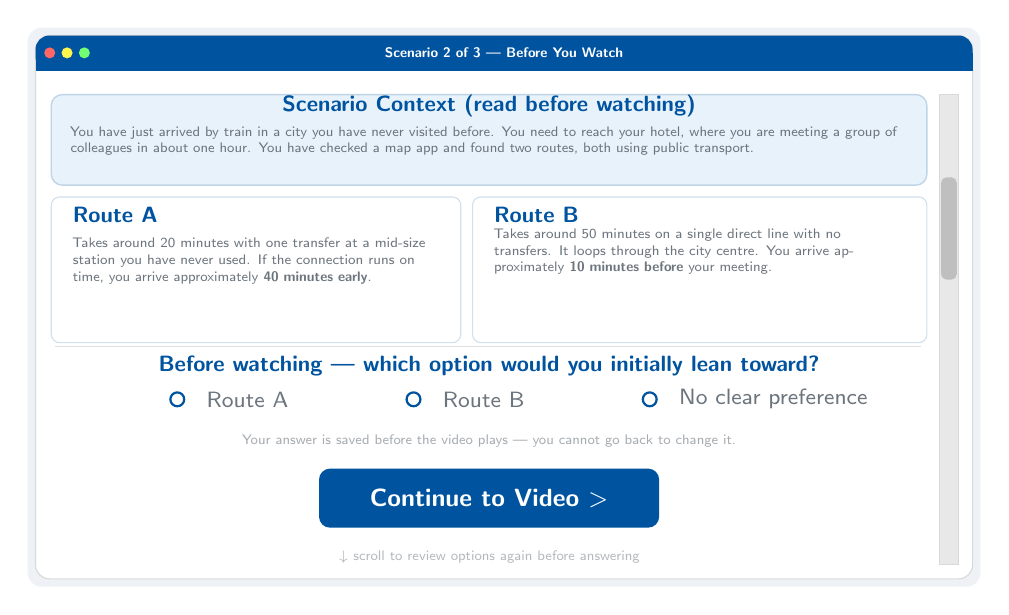
\begin{tikzpicture}[x=1cm, y=1cm]

  \browserchrome{0.4}{0.0}{12.3}{6.9}{Scenario 2 of 3 --- Before You Watch}
  %\progressbar{0.9}{6.38}{11.8}{0.38}{Step 3 of 8}

  \fill[gray!18] (11.88,0.18) rectangle (12.12,6.15);
  \draw[gray!30, line width=0.3pt] (11.88,0.18) rectangle (12.12,6.15);
  \fill[gray!50, rounded corners=2pt] (11.90,3.80) rectangle (12.10,5.10);
  \node[font=\tiny\color{gray!55}] at (12.0,6.05) {$\scriptstyle\blacktriangle$};
  \node[font=\tiny\color{gray!55}] at (12.0,0.28) {$\scriptstyle\blacktriangledown$};

  \fill[kbluelight, draw=kblue!25, rounded corners=4pt, line width=0.5pt]
    (0.60,5.00) rectangle (11.72,6.15);
  \node[font=\footnotesize\sffamily\bfseries\color{kblue}] at (6.16,6.0)
    {Scenario Context (read before watching)};
  \node[font=\tiny\sffamily\color{kgray}, text width=10.5cm, anchor=north west]
    at (0.72,5.87)
    {You have just arrived by train in a city you have never visited before. You need
     to reach your hotel, where you are meeting a group of colleagues in about one hour.
     You have checked a map app and found two routes, both using public transport.};

  \fill[white, draw=kblue!18, rounded corners=3pt, line width=0.4pt]
    (0.60,3) rectangle (5.80,4.85);
  \node[font=\footnotesize\sffamily\bfseries\color{kblue}, anchor=north west] at (0.75,4.85)
    {Route A};
  \node[font=\tiny\sffamily\color{kgray}, text width=4.7cm, anchor=north west]
    at (0.75,4.45)
    {Takes around 20 minutes with one transfer at a mid-size station you have never used.
     If the connection runs on time, you arrive approximately \textbf{40 minutes early}.};

  \fill[white, draw=kblue!18, rounded corners=3pt, line width=0.4pt]
    (5.95,3) rectangle (11.72,4.85);
  \node[font=\footnotesize\sffamily\bfseries\color{kblue}, anchor=north west] at (6.10,4.85)
    {Route B};
  \node[font=\tiny\sffamily\color{kgray}, text width=4.7cm, anchor=north west]
    at (6.10,4.57)
    {Takes around 50 minutes on a single direct line with no transfers.
     It loops through the city centre. You arrive approximately \textbf{10 minutes before} your meeting.};

  \draw[gray!25, line width=0.3pt] (0.65,2.95) -- (11.65,2.95);

  \node[font=\footnotesize\sffamily\bfseries\color{kblue}] at (6.16,2.7)
    {Before watching --- which option would you initially lean toward?};

  \node[radio] at (2.2,2.28) {};
  \node[font=\footnotesize\sffamily\color{kgray}, anchor=west] at (2.45,2.28) {Route A};
  \node[radio] at (5.2,2.28) {};
  \node[font=\footnotesize\sffamily\color{kgray}, anchor=west] at (5.45,2.28) {Route B};
  \node[radio] at (8.2,2.28) {};
  \node[font=\footnotesize\sffamily\color{kgray}, anchor=west] at (8.45,2.28)
    {No clear preference};

  \node[font=\tiny\sffamily\color{kgray!60}] at (6.16,1.75)
    {Your answer is saved before the video plays --- you cannot go back to change it.};

  \fill[kblue, rounded corners=4pt] (4.0,0.65) rectangle (8.32,1.40);
  \node[font=\small\sffamily\bfseries, text=white] at (6.16,1.02)
    {Continue to Video \textbf{\textgreater}};

  \node[font=\tiny\sffamily\color{kgray!50}, align=center] at (6.16,0.28)
    {$\downarrow$ scroll to review options again before answering};

\end{tikzpicture}
\end{center}
\end{frame}

%% ═══════════════════════════════════════════════════════════════════════════
%% SCENE 3c — Scenario Detail: Learning Resource
%% ═══════════════════════════════════════════════════════════════════════════
\begin{frame}{Scene 3c — Scenario Page (Learning Resource)}
\begin{center}
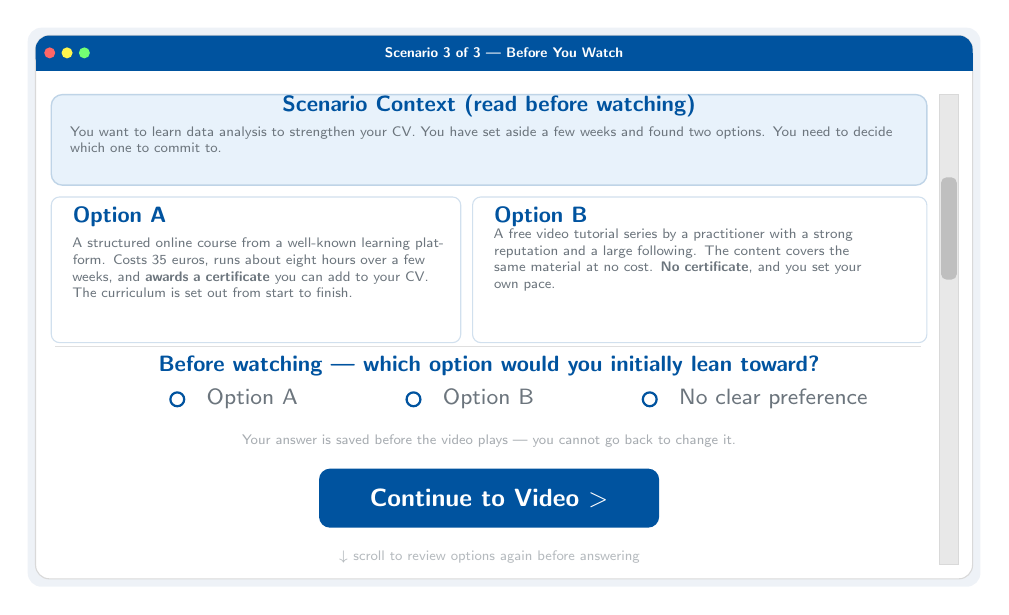
\begin{tikzpicture}[x=1cm, y=1cm]

  \browserchrome{0.4}{0.0}{12.3}{6.9}{Scenario 3 of 3 --- Before You Watch}
  %\progressbar{0.9}{6.38}{11.8}{0.38}{Step 3 of 8}

  \fill[gray!18] (11.88,0.18) rectangle (12.12,6.15);
  \draw[gray!30, line width=0.3pt] (11.88,0.18) rectangle (12.12,6.15);
  \fill[gray!50, rounded corners=2pt] (11.90,3.80) rectangle (12.10,5.10);
  \node[font=\tiny\color{gray!55}] at (12.0,6.05) {$\scriptstyle\blacktriangle$};
  \node[font=\tiny\color{gray!55}] at (12.0,0.28) {$\scriptstyle\blacktriangledown$};

  \fill[kbluelight, draw=kblue!25, rounded corners=4pt, line width=0.5pt]
    (0.60,5.00) rectangle (11.72,6.15);
  \node[font=\footnotesize\sffamily\bfseries\color{kblue}] at (6.16,6.0)
    {Scenario Context (read before watching)};
  \node[font=\tiny\sffamily\color{kgray}, text width=10.5cm, anchor=north west]
    at (0.72,5.87)
    {You want to learn data analysis to strengthen your CV. You have set aside a few weeks
     and found two options. You need to decide which one to commit to.};

  \fill[white, draw=kblue!18, rounded corners=3pt, line width=0.4pt]
    (0.60,3) rectangle (5.80,4.85);
  \node[font=\footnotesize\sffamily\bfseries\color{kblue}, anchor=north west] at (0.75,4.85)
    {Option A};
  \node[font=\tiny\sffamily\color{kgray}, text width=4.7cm, anchor=north west]
    at (0.75,4.45)
    {A structured online course from a well-known learning platform. Costs 35 euros,
     runs about eight hours over a few weeks, and \textbf{awards a certificate} you can add to your CV.
     The curriculum is set out from start to finish.};

  \fill[white, draw=kblue!18, rounded corners=3pt, line width=0.4pt]
    (5.95,3) rectangle (11.72,4.85);
  \node[font=\footnotesize\sffamily\bfseries\color{kblue}, anchor=north west] at (6.10,4.85)
    {Option B};
  \node[font=\tiny\sffamily\color{kgray}, text width=4.7cm, anchor=north west]
    at (6.10,4.57)
    {A free video tutorial series by a practitioner with a strong reputation and a large following.
     The content covers the same material at no cost. \textbf{No certificate}, and you set your own pace.};

  \draw[gray!25, line width=0.3pt] (0.65,2.95) -- (11.65,2.95);

  \node[font=\footnotesize\sffamily\bfseries\color{kblue}] at (6.16,2.7)
    {Before watching --- which option would you initially lean toward?};

  \node[radio] at (2.2,2.28) {};
  \node[font=\footnotesize\sffamily\color{kgray}, anchor=west] at (2.45,2.28) {Option A};
  \node[radio] at (5.2,2.28) {};
  \node[font=\footnotesize\sffamily\color{kgray}, anchor=west] at (5.45,2.28) {Option B};
  \node[radio] at (8.2,2.28) {};
  \node[font=\footnotesize\sffamily\color{kgray}, anchor=west] at (8.45,2.28)
    {No clear preference};

  \node[font=\tiny\sffamily\color{kgray!60}] at (6.16,1.75)
    {Your answer is saved before the video plays --- you cannot go back to change it.};

  \fill[kblue, rounded corners=4pt] (4.0,0.65) rectangle (8.32,1.40);
  \node[font=\small\sffamily\bfseries, text=white] at (6.16,1.02)
    {Continue to Video \textbf{\textgreater}};

  \node[font=\tiny\sffamily\color{kgray!50}, align=center] at (6.16,0.28)
    {$\downarrow$ scroll to review options again before answering};

\end{tikzpicture}
\end{center}
\end{frame}


% %% ═══════════════════════════════════════════════════════════════════════════
% %% SLIDE 6 — Scene 2: Vignette + Baseline (compact view for flow context)
% %% ═══════════════════════════════════════════════════════════════════════════
% \begin{frame}{Scene 2 — Scenario Vignette + Baseline Question}
% \begin{center}
% \begin{tikzpicture}[x=1cm, y=1cm]

%   \browserchrome{1.0}{0.2}{13.0}{6.8}{Scenario [N] of 3 --- Before You Watch}
%   \progressbar{1.5}{6.2}{12.5}{0.38}{Step 3 of 8}

%   %% Scenario box
%   \fill[kbluelight, rounded corners=4pt] (1.5,2.85) rectangle (12.5,5.9);
%   \draw[kblue!25, rounded corners=4pt, line width=0.5pt] (1.5,2.85) rectangle (12.5,5.9);
%   \node[font=\tiny\sffamily\bfseries\color{kblue}] at (7.0,5.72)
%     {Scenario Context (read before watching)};
%   \node[font=\tiny\sffamily\color{kgray}, text width=9.6cm, anchor=north west]
%     at (1.65,5.60)
%     {Full vignette text describing the decision situation and \textbf{both options
%      with equal detail.} Participants read this before the video plays.};

%   %% Option A row (taller: bottom from 4.5 to 4.0; label font reduced from \small to \footnotesize)
%   \fill[white, rounded corners=2pt] (1.75,4.0) rectangle (6.85,5.05);
%   \node[font=\footnotesize\sffamily\bfseries\color{kblue}, anchor=north west] at (1.88,5.02)
%     {Option A};
%   \node[font=\tiny\sffamily\color{kgray}, text width=4.5cm, anchor=north west]
%     at (1.88,4.65)
%     {Full description with advantages and trade-offs stated objectively.};

%   %% Option B row (same fix)
%   \fill[white, rounded corners=2pt] (7.05,4.0) rectangle (12.25,5.05);
%   \node[font=\footnotesize\sffamily\bfseries\color{kblue}, anchor=north west] at (7.18,5.02)
%     {Option B};
%   \node[font=\tiny\sffamily\color{kgray}, text width=4.5cm, anchor=north west]
%     at (7.18,4.65)
%     {Full description with advantages and trade-offs stated objectively.};

%   \draw[kblue!20, line width=0.3pt] (1.65,3.80) -- (12.35,3.80);
%   \node[font=\tiny\sffamily\itshape\color{kgray!70}, align=center, text width=9.5cm]
%     at (7.0,3.40)
%     {The advisor's video will give only their recommendation and reasoning.
%      They will not re-describe the options above.};

%   %% Baseline question
%   \node[font=\footnotesize\sffamily\bfseries\color{kgray}, text width=10.5cm, align=center] at (7.0,2.55)
%     {Based only on the situation described above, before watching the video, which option would you initially lean toward?};

%   \node[radio] at (3.0,2.1) {};
%   \node[font=\footnotesize\sffamily\color{kgray}, anchor=west] at (3.2,2.1) {Option A};
%   \node[radio] at (6.2,2.1) {};
%   \node[font=\footnotesize\sffamily\color{kgray}, anchor=west] at (6.4,2.1) {Option B};
%   \node[radio] at (9.4,2.1) {};
%   \node[font=\footnotesize\sffamily\color{kgray}, anchor=west] at (9.6,2.1)
%     {No clear preference};

%   \node[font=\tiny\sffamily\color{kgray!60}, text width=10cm, align=center] at (7.0,1.70)
%     {Options vary per scenario: Job A/B · Route A/B · Option A/B. ``No clear preference'' always available.};

%   \fill[kblue, rounded corners=4pt] (5.0,0.8) rectangle (9.0,1.45);
%   \node[font=\small\sffamily\bfseries, text=white] at (7.0,1.12)
%     {Continue to Video \textbf{\textgreater}};

% \end{tikzpicture}
% \end{center}
% \end{frame}

% %% ═══════════════════════════════════════════════════════════════════════════
% %% SLIDE 7 — Scene 3: Video Stimulus
% %% ═══════════════════════════════════════════════════════════════════════════
% \begin{frame}{Scene 3 — Video Stimulus \textnormal{\small (advisor speaks recommendation only,
%   \textasciitilde 55 s)}}
% \begin{center}
% \begin{tikzpicture}[x=1cm, y=1cm]

%   \browserchrome{1.0}{0.2}{13.0}{6.8}{Video 1 of 3}
%   \progressbar{1.5}{6.2}{12.5}{0.50}{Step 4 of 8}

%   %% Large video placeholder
%   \fill[vidbox] (2.0,0.8) rectangle (12.0,5.7);
%   \draw[gray!40, rounded corners=3pt] (2.0,0.8) rectangle (12.0,5.7);

%   %% Play button
%   \fill[white, opacity=0.75] (7.0,3.25) circle (0.8);
%   \fill[kblue!80] (6.65,2.85) -- (6.65,3.65) -- (7.55,3.25) -- cycle;

%   %% Duration badge
%   \fill[black!55, rounded corners=2pt] (10.8,1.0) rectangle (11.9,1.4);
%   \node[font=\tiny\sffamily, text=white] at (11.35,1.2) {0:55};

%   %% Condition corner badge
%   \fill[kbluedark, opacity=0.75, rounded corners=2pt] (2.1,5.4) rectangle (4.0,5.65);
%   \node[font=\tiny\sffamily, text=white] at (3.05,5.52) {C1 / C2 / C3};

%   \node[font=\tiny\sffamily\color{kgray}] at (7.0,0.5)
%     {Please watch the full video before continuing.
%      \quad The video cannot be paused or replayed.};

% \end{tikzpicture}
% \end{center}
% \end{frame}

% %% ═══════════════════════════════════════════════════════════════════════════
% %% SLIDE 8 — Scene 4: Post-Video Questionnaire
% %% ═══════════════════════════════════════════════════════════════════════════
% \begin{frame}{Scene 4 — Post-Video Questionnaire}
% \begin{center}
% \begin{tikzpicture}[x=1cm, y=1cm]

%   \browserchrome{0.4}{0.1}{13.6}{6.9}{Questions --- Video 1 of 3}
%   \progressbar{0.9}{6.4}{13.1}{0.62}{Step 5 of 8}

%   %% A. Comprehension Check
%   \node[font=\tiny\sffamily\bfseries\color{kblue}, anchor=west] at (0.7,5.9)
%     {A. \; Comprehension Check};
%   \node[font=\tiny\sffamily\color{kgray}, anchor=west] at (0.7,5.6)
%     {What did the advisor recommend? \quad
%      $\circ$\ Option A \quad $\circ$\ Option B \quad
%      $\circ$\ I did not watch the full video};
%   \draw[gray!20, line width=0.3pt] (0.7,5.35) -- (13.3,5.35);

%   %% B. Eeriness
%   \node[font=\tiny\sffamily\bfseries\color{kblue}, anchor=west] at (0.7,5.15)
%     {B. \; Eeriness --- strangeness / discomfort \textnormal{(Ho \& MacDorman, 2010)}};
%   \fill[klightgray, rounded corners=2pt] (0.7,4.50) rectangle (13.3,5.05);
%   \node[font=\tiny\sffamily\color{kgray}, anchor=west] at (0.8,4.85) {Not at all eerie};
%   \foreach \i in {0,1,2,3,4} { \draw[gray!50] ({4.5+\i*0.5},4.78) circle (0.09); }
%   \node[font=\tiny\sffamily\color{kgray}, anchor=west] at (7.2,4.85) {Very eerie};
%   \node[font=\tiny\sffamily\color{kgray!60}, anchor=west] at (0.8,4.58)
%     {+ 5 more items (6 total)};
%   \draw[gray!20, line width=0.3pt] (0.7,4.30) -- (13.3,4.30);

%   %% C. Likeability
%   \node[font=\tiny\sffamily\bfseries\color{kblue}, anchor=west] at (0.7,4.10)
%     {C. \; Likeability \textnormal{(Godspeed --- Bartneck et al., 2009)}};
%   \fill[klightgray, rounded corners=2pt] (0.7,3.55) rectangle (13.3,4.0);
%   \node[font=\tiny\sffamily\color{kgray}, anchor=west] at (0.8,3.78) {Dislike};
%   \foreach \i in {0,1,2,3,4} { \draw[gray!50] ({4.5+\i*0.5},3.78) circle (0.09); }
%   \node[font=\tiny\sffamily\color{kgray}, anchor=west] at (7.2,3.78)
%     {Like \quad + 4 more items};
%   \draw[gray!20, line width=0.3pt] (0.7,3.35) -- (13.3,3.35);

%   %% D. Anthropomorphism
%   \node[font=\tiny\sffamily\bfseries\color{kblue}, anchor=west] at (0.7,3.15)
%     {D. \; Human-Likeness \textnormal{(Godspeed --- Bartneck et al., 2009)}};
%   \fill[klightgray, rounded corners=2pt] (0.7,2.58) rectangle (13.3,3.05);
%   \node[font=\tiny\sffamily\color{kgray}, anchor=west] at (0.8,2.82)
%     {Machinelike};
%   \foreach \i in {0,1,2,3,4} { \draw[gray!50] ({4.5+\i*0.5},2.82) circle (0.09); }
%   \node[font=\tiny\sffamily\color{kgray}, anchor=west] at (7.2,2.82)
%     {Humanlike \quad + 4 more items};
%   \draw[gray!20, line width=0.3pt] (0.7,2.38) -- (13.3,2.38);

%   %% E-G. Trust
%   \node[font=\tiny\sffamily\bfseries\color{kblue}, anchor=west] at (0.7,2.18)
%     {E--G. \; Trust: Competence \textbullet\ Benevolence \textbullet\ Integrity
%      \quad (7-point Likert, Canales et al., 2024)};
%   \fill[klightgray, rounded corners=2pt] (0.7,1.62) rectangle (13.3,2.08);
%   \node[font=\tiny\sffamily\color{kgray}, anchor=west] at (0.8,1.85)
%     {I believe this advisor is capable and competent.};
%   \foreach \i in {0,1,2,3,4,5,6} { \draw[gray!50] ({7.5+\i*0.43},1.85) circle (0.08); }
%   \node[font=\tiny\sffamily\color{kgray!60}, anchor=west] at (0.8,1.65)
%     {+ 10 more items across 3 subscales};
%   \draw[gray!20, line width=0.3pt] (0.7,1.45) -- (13.3,1.45);

%   %% H. Recommendation agreement + Warmth
%   \node[font=\tiny\sffamily\bfseries\color{kblue}, anchor=west] at (0.7,1.28)
%     {H. \; Recommendation Agreement \textbullet\ Warmth \quad (7-point Likert)};
%   \fill[klightgray, rounded corners=2pt] (0.7,0.82) rectangle (13.3,1.18);
%   \node[font=\tiny\sffamily\color{kgray}, anchor=west] at (0.8,1.00)
%     {I agree with the recommendation this advisor gave.};
%   \foreach \i in {0,1,2,3,4,5,6} { \draw[gray!50] ({7.5+\i*0.43},1.00) circle (0.08); }
%   \draw[gray!20, line width=0.3pt] (0.7,0.65) -- (13.3,0.65);

%   %% I + AC. Manipulation check + Attention check
%   \node[font=\tiny\sffamily\bfseries\color{kblue}, anchor=west] at (0.7,0.50)
%     {I. \; Visual Style Check \textnormal{(manip.\ check, 1--7)}
%      \quad \textbf{AC.} Attention check \textnormal{(target varies per block: 3 / 4 / 2)}};

%   %% Next button
%   \fill[kblue, rounded corners=3pt] (11.0,0.08) rectangle (13.3,0.38);
%   \node[font=\small\sffamily\bfseries, text=white] at (12.15,0.23)
%     {Next \textbf{\textgreater}};

% \end{tikzpicture}
% \end{center}
% \end{frame}

%% ═══════════════════════════════════════════════════════════════════════════
%% SCENE 4-DETAIL-A — Per-Block Overview + Pre-Video + Part A
%% ═══════════════════════════════════════════════════════════════════════════
\begin{frame}{Scene 4  --- Block Structure \& Part A Comprehension Check}
\begin{center}
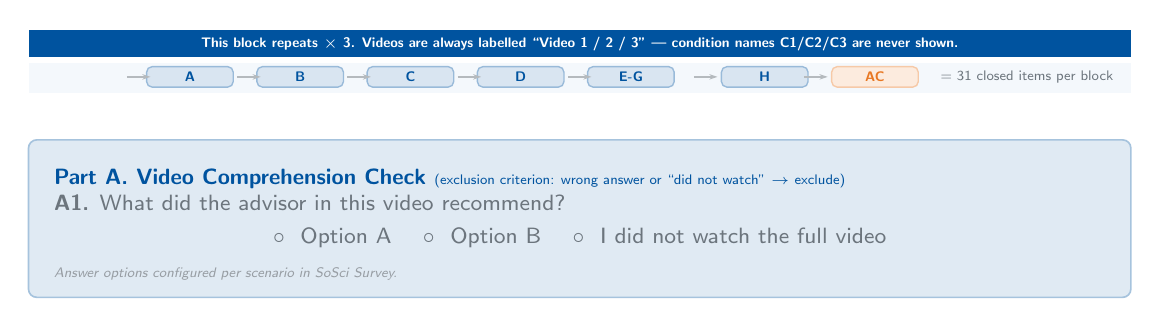
\begin{tikzpicture}[x=1cm, y=1cm]

  %% Block order header
  \fill[kblue] (0.0,6.55) rectangle (14.0,6.90);
  \node[font=\tiny\sffamily\bfseries, text=white] at (7.0,6.72)
    {This block repeats $\times$ 3. Videos are always labelled ``Video 1 / 2 / 3'' — condition names C1/C2/C3 are never shown.};

  %% Order boxes
  \fill[kbluepale] (0.0,6.10) rectangle (14.0,6.48);
  %% A-H boxes (kblue)
  \foreach \xpos/\lab in {2.05/A, 3.45/B, 4.85/C, 6.25/D, 7.65/{E-G}, 9.35/H}{
    \fill[kblue!15, rounded corners=2pt] ({\xpos-0.55},6.17) rectangle ({\xpos+0.55},6.43);
    \draw[kblue!40, rounded corners=2pt, line width=0.5pt] ({\xpos-0.55},6.17) rectangle ({\xpos+0.55},6.43);
    \node[font=\tiny\sffamily\bfseries\color{kblue}] at (\xpos,6.30) {\lab};
  }
  %% AC box (orange)
  \fill[korange!15, rounded corners=2pt] (10.20,6.17) rectangle (11.30,6.43);
  \draw[korange!40, rounded corners=2pt, line width=0.5pt] (10.20,6.17) rectangle (11.30,6.43);
  \node[font=\tiny\sffamily\bfseries\color{korange}] at (10.75,6.30) {AC};
  %% Arrows between boxes
  \foreach \x in {1.25,2.65,4.05,5.45,6.85,8.45,9.85} {
    \draw[kgray!50, -{Stealth[length=3pt,width=2pt]}, line width=0.5pt] (\x,6.30) -- ({\x+0.30},6.30);
  }
  \node[font=\tiny\sffamily\color{kgray}, anchor=east] at (13.9,6.30)
    {= 31 closed items per block};

  %% PART A
  \fill[kblue!12, rounded corners=3pt] (0.0,5.50) rectangle (14.0,3.50);
  \draw[kblue!35, rounded corners=3pt, line width=0.6pt] (0.0,5.50) rectangle (14.0,3.5);
  \node[font=\footnotesize\sffamily\bfseries\color{kblue}, anchor=west] at (0.2,5.)
    {Part A. Video Comprehension Check \textnormal{\tiny (exclusion criterion: wrong answer or ``did not watch'' $\to$ exclude)}};
  \node[font=\footnotesize\sffamily\color{kgray}, anchor=west] at (0.2,4.7)
    {\textbf{A1.} What did the advisor in this video recommend?};
  \node[font=\footnotesize\sffamily\color{kgray}] at (7.0,4.25)
    {$\circ$ \ Option A \quad $\circ$ \ Option B \quad $\circ$ \ I did not watch the full video};
  \node[font=\tiny\sffamily\color{kgray!70}, anchor=west] at (0.2,3.8)
    {\textit{Answer options configured per scenario in SoSci Survey.}};

  % %% Scale structure summary boxes
  % \fill[kbluepale, rounded corners=3pt] (0.0,0.12) rectangle (14.0,3.12);
  % \node[font=\footnotesize\sffamily\bfseries\color{kblue}] at (7.0,2.95) {Question structure after Part A};

  % % 5-point block
  % \fill[kblue!18, rounded corners=3pt] (0.1,1.80) rectangle (6.8,2.78);
  % \node[font=\footnotesize\sffamily\bfseries\color{kblue}] at (3.45,2.62)
  %   {5-point Semantic Differential};
  % \node[font=\footnotesize\sffamily\color{kblue!80}] at (1.1,2.32) {\textbf{B.} Eeriness};
  % \node[font=\tiny\sffamily\color{kgray}] at (1.1,2.12) {6 items};
  % \node[font=\tiny\sffamily\color{kgray}] at (1.1,1.96) {Ho \& MacDorman};
  % \node[font=\footnotesize\sffamily\color{kblue!80}] at (3.45,2.32) {\textbf{C.} Likeability};
  % \node[font=\tiny\sffamily\color{kgray}] at (3.45,2.12) {5 items};
  % \node[font=\tiny\sffamily\color{kgray}] at (3.45,1.96) {Godspeed};
  % \node[font=\footnotesize\sffamily\color{kblue!80}] at (5.75,2.32) {\textbf{D.} Human-Likeness};
  % \node[font=\tiny\sffamily\color{kgray}] at (5.75,2.12) {5 items};
  % \node[font=\tiny\sffamily\color{kgray}] at (5.75,1.96) {Godspeed};

  % % scale change separator
  % \fill[korange!15, rounded corners=2pt] (0.1,1.52) rectangle (6.8,1.76);
  % \node[font=\tiny\sffamily\bfseries\color{korange!80!black}] at (3.45,1.64)
  %   {$\longrightarrow$ Scale change shown to participants: 1--7, SD to SA};

  % % 7-point block
  % \fill[kblue!18, rounded corners=3pt] (7.2,1.52) rectangle (13.9,2.78);
  % \node[font=\footnotesize\sffamily\bfseries\color{kblue}] at (10.55,2.62)
  %   {7-point Likert (1 = SD, 7 = SA)};
  % \node[font=\footnotesize\sffamily\color{kblue!80}] at (8.0,2.32) {\textbf{E.} Competence};
  % \node[font=\tiny\sffamily\color{kgray}] at (8.0,2.04) {4 items};
  % \node[font=\footnotesize\sffamily\color{kblue!80}] at (9.4,2.32) {\textbf{F.} Benevolence};
  % \node[font=\tiny\sffamily\color{kgray}] at (9.4,2.04) {4 items};
  % \node[font=\footnotesize\sffamily\color{kblue!80}] at (10.8,2.32) {\textbf{G.} Integrity};
  % \node[font=\tiny\sffamily\color{kgray}] at (10.8,2.04) {3 items};
  % \node[font=\footnotesize\sffamily\color{kblue!80}] at (12.2,2.32) {\textbf{H.} Agreement};
  % \node[font=\tiny\sffamily\color{kgray}] at (12.2,2.04) {+ Warmth};
  % \node[font=\tiny\sffamily\color{kgray}] at (12.2,1.88) {2 items};

  % % AC row
  % \fill[korange!15, rounded corners=3pt] (0.1,0.20) rectangle (13.9,1.44);
  % \draw[korange!40, rounded corners=3pt, line width=0.6pt] (0.1,0.20) rectangle (13.9,1.44);
  % \node[font=\footnotesize\sffamily\bfseries\color{korange}] at (7.0,1.27)
  %   {AC. Attention Check \textnormal{\small (embedded once per block; target varies)}};
  % \node[font=\footnotesize\sffamily\color{kgray}] at (7.0,1.02)
  %   {``To confirm you are reading carefully, please select option [N].''};
  % \node[font=\footnotesize\sffamily\color{kgray}] at (7.0,0.72)
  %   {Block 1: select \textbf{3} \quad\quad Block 2: select \textbf{4} \quad\quad Block 3: select \textbf{2}};
  % \node[font=\tiny\sffamily\color{kgray!70}] at (7.0,0.38) {Exclude participants who fail any one check.};

\end{tikzpicture}
\end{center}
\end{frame}

%% ═══════════════════════════════════════════════════════════════════════════
%% SCENE 4-DETAIL-B — Part D: Eeriness (6 items)
%% ═══════════════════════════════════════════════════════════════════════════
%% ═══════════════════════════════════════════════════════════════════════════
%% SCENE 4-DETAIL-B/C — Parts B & C: Likeability + Human-Likeness (5+5 items)
%% ═══════════════════════════════════════════════════════════════════════════
\begin{frame}{Scene 5 --- Parts B \& C: Likeability + Human-Likeness \textnormal{\small (Godspeed)}}
\begin{center}
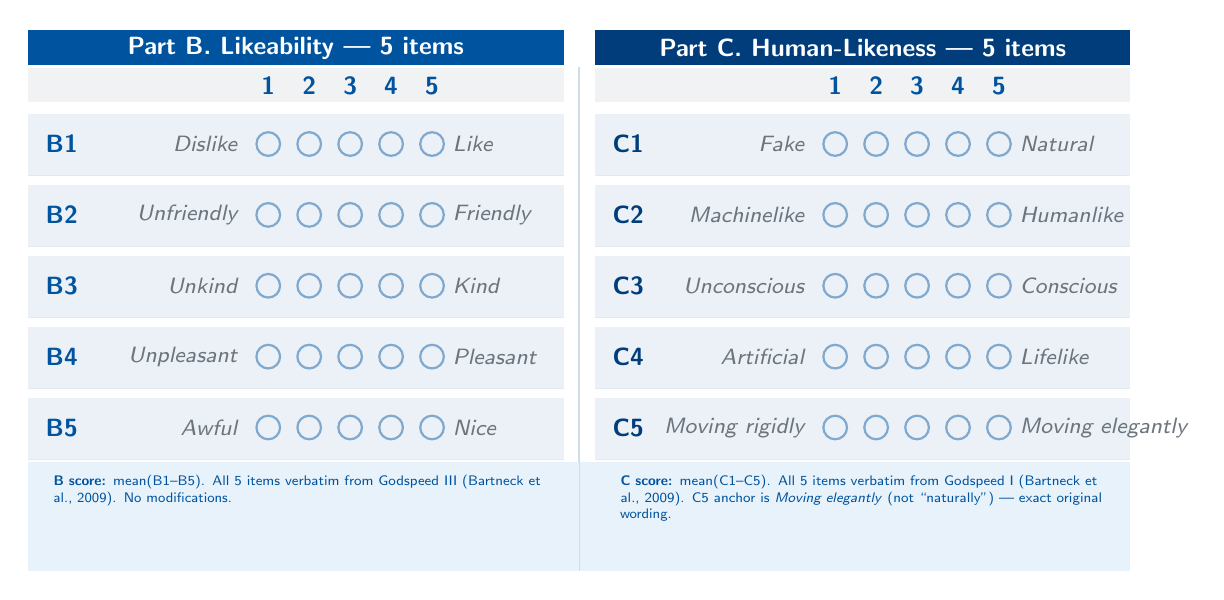
\begin{tikzpicture}[x=1cm, y=1cm]

  %% Part B header
  \fill[kblue] (0.0,6.50) rectangle (6.8,6.95);
  \node[font=\small\sffamily\bfseries, text=white] at (3.4,6.72)
    {Part B. Likeability --- 5 items};

  %% Part C header
  \fill[kbluedark] (7.2,6.50) rectangle (14.0,6.95);
  \node[font=\small\sffamily\bfseries, text=white] at (10.6,6.72)
    {Part C. Human-Likeness --- 5 items};

  %% Scale headers
  \fill[klightgray] (0.0,6.03) rectangle (6.8,6.46);
  \fill[klightgray] (7.2,6.03) rectangle (14.0,6.46);
  \foreach \xoff in {0.0, 7.2}{
    \foreach \i/\n in {0/1,1/2,2/3,3/4,4/5}{
      \node[font=\small\sffamily\bfseries\color{kblue}] at ({\xoff+3.05+\i*0.52},6.24) {\n};
    }
  }

  %% Vertical divider
  \draw[kblue!20, line width=0.6pt] (7.0,0.08) -- (7.0,6.48);

  %% Part B items (5 items — Likeability)
  \foreach \y/\itnum/\la/\ra in {
    5.5/B1/Dislike/Like,
    4.6/B2/Unfriendly/Friendly,
    3.7/B3/Unkind/Kind,
    2.8/B4/Unpleasant/Pleasant,
    1.9/B5/Awful/Nice
  }{
    \fill[kblue!8] (0.0,{\y-0.40}) rectangle (6.8,{\y+0.38});
    \draw[kblue!12, line width=0.3pt] (0.0,{\y-0.40}) -- (6.8,{\y-0.40});
    \node[font=\small\sffamily\bfseries\color{kblue}, anchor=west] at (0.1,\y) {\itnum};
    \node[font=\footnotesize\sffamily\itshape\color{kgray}, anchor=east] at (2.78,\y) {\la};
    \foreach \i in {0,1,2,3,4}{
      \draw[kblue!50, line width=0.8pt] ({3.05+\i*0.52},\y) circle (0.15);
    }
    \node[font=\footnotesize\sffamily\itshape\color{kgray}, anchor=west] at (5.27,\y) {\ra};
  }

  %% Part C items (5 items — Anthropomorphism)
  \foreach \y/\itnum/\la/\ra in {
    5.5/C1/Fake/Natural,
    4.6/C2/Machinelike/Humanlike,
    3.7/C3/Unconscious/Conscious,
    2.8/C4/Artificial/Lifelike,
    1.9/C5/{Moving rigidly}/{Moving elegantly}
  }{
    \fill[kblue!8] (7.2,{\y-0.40}) rectangle (14.0,{\y+0.38});
    \draw[kblue!12, line width=0.3pt] (7.2,{\y-0.40}) -- (14.0,{\y-0.40});
    \node[font=\small\sffamily\bfseries\color{kbluedark}, anchor=west] at (7.3,\y) {\itnum};
    \node[font=\footnotesize\sffamily\itshape\color{kgray}, anchor=east] at (9.98,\y) {\la};
    \foreach \i in {0,1,2,3,4}{
      \draw[kblue!50, line width=0.8pt] ({10.25+\i*0.52},\y) circle (0.15);
    }
    \node[font=\footnotesize\sffamily\itshape\color{kgray}, anchor=west] at (12.47,\y) {\ra};
  }

  %% Footer
  \fill[kbluelight] (0.0,0.08) rectangle (14.0,1.46);
  \draw[kblue!20, line width=0.3pt] (7.0,0.08) -- (7.0,1.46);
  \node[font=\tiny\sffamily\color{kblue}, text width=6.3cm, anchor=north west] at (0.2,1.42)
    {\textbf{B score:} mean(B1--B5). All 5 items verbatim from Godspeed III (Bartneck et al., 2009). No modifications.};
  \node[font=\tiny\sffamily\color{kblue}, text width=6.3cm, anchor=north west] at (7.4,1.42)
    {\textbf{C score:} mean(C1--C5). All 5 items verbatim from Godspeed I (Bartneck et al., 2009). C5 anchor is \textit{Moving elegantly} (not ``naturally'') --- exact original wording.};

\end{tikzpicture}
\end{center}
\end{frame}

\begin{frame}{Scene 6 --- Part D: Eeriness \textnormal{\small (Ho \& MacDorman, 2010 --- 8 items verbatim, 5-point)}}
\begin{center}
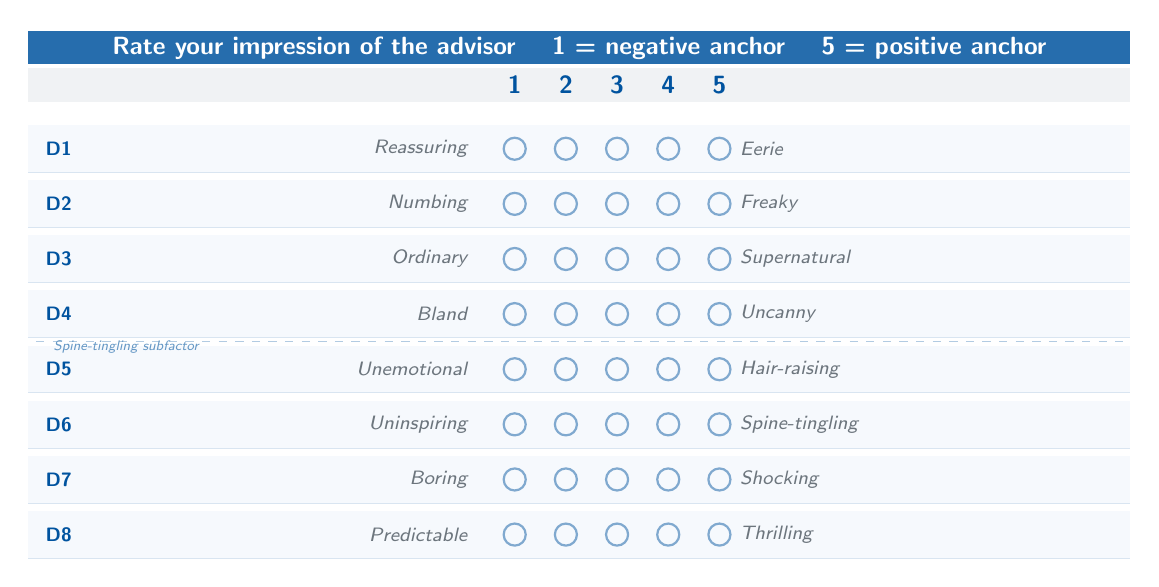
\begin{tikzpicture}[x=1cm, y=1cm]

  %% Part D header
  \fill[kblue!85] (0.0,6.52) rectangle (14.0,6.95);
  \node[font=\small\sffamily\bfseries, text=white] at (7.0,6.73)
    {Rate your impression of the advisor \quad 1 = negative anchor \quad 5 = positive anchor};

  %% Scale column headers
  \fill[klightgray] (0.0,6.05) rectangle (14.0,6.48);
  \foreach \i/\n in {0/1,1/2,2/3,3/4,4/5} {
    \node[font=\small\sffamily\bfseries\color{kblue}] at ({6.18+\i*0.65},6.26) {\n};
  }

  %% Sem-diff items (Part D — Eeriness, 8 verbatim items from Ho & MacDorman 2010)
  %% Eerie subfactor: D1-D4 | Spine-tingling subfactor: D5-D8
  \foreach \y/\itnum/\la/\ra in {
    5.45/D1/{Reassuring}/{Eerie},
    4.75/D2/{Numbing}/{Freaky},
    4.05/D3/{Ordinary}/{Supernatural},
    3.35/D4/{Bland}/{Uncanny},
    2.65/D5/{Unemotional}/{Hair-raising},
    1.95/D6/{Uninspiring}/{Spine-tingling},
    1.25/D7/{Boring}/{Shocking},
    0.55/D8/{Predictable}/{Thrilling}
  }{
    \fill[kbluepale!80] (0.0,{\y-0.30}) rectangle (14.0,{\y+0.30});
    \draw[kblue!15, line width=0.3pt] (0.0,{\y-0.30}) -- (14.0,{\y-0.30});
    \node[font=\scriptsize\sffamily\bfseries\color{kblue}, anchor=west] at (0.1,\y) {\itnum};
    \node[font=\scriptsize\sffamily\itshape\color{kgray}, anchor=east, text width=4.5cm, align=right]
      at (5.70,\y) {\la};
    \foreach \i in {0,1,2,3,4}{
      \draw[kblue!50, line width=0.8pt] ({6.18+\i*0.65},\y) circle (0.14);
    }
    \node[font=\scriptsize\sffamily\itshape\color{kgray}, anchor=west, text width=4.5cm]
      at (8.92,\y) {\ra};
  }
  %% Subfactor divider
  \draw[kblue!30, line width=0.6pt, dashed] (0.1,3.00) -- (13.9,3.00);
  \node[font=\tiny\sffamily\color{kblue!60}, anchor=west] at (0.2,2.93)
    {\textit{Spine-tingling subfactor}};

\end{tikzpicture}
\end{center}
\end{frame}

%% ═══════════════════════════════════════════════════════════════════════════
%% SCENE 4-DETAIL-D-E — Part E: Trust Competence (4 items)
%% ═══════════════════════════════════════════════════════════════════════════
\begin{frame}{Scene 7 --- Part E: Trust Competence \textnormal{\small (Canales et al., 2024 --- 4 items, 7-point Likert)}}
\begin{center}
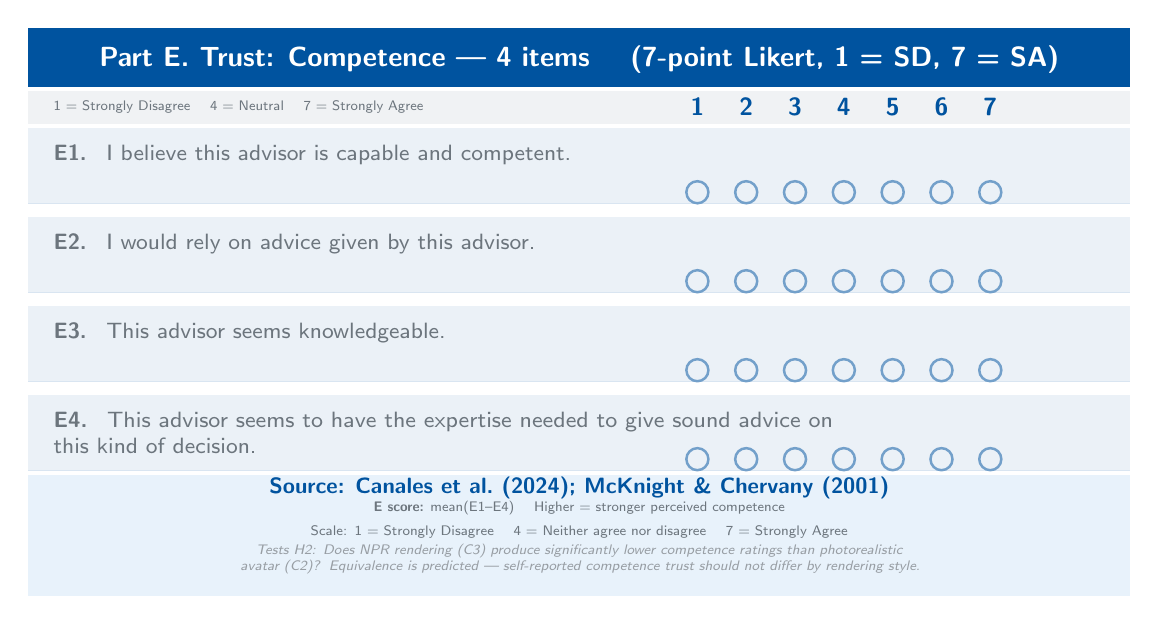
\begin{tikzpicture}[x=1cm, y=1cm]

  %% Header
  \fill[kblue] (0.0,6.55) rectangle (14.0,7.3);
  \node[font=\normalsize\sffamily\bfseries, text=white] at (7.0,6.9)
    {Part E. Trust: Competence --- 4 items \quad (7-point Likert, 1 = SD, 7 = SA)};

  %% Scale bar
  \fill[klightgray] (0.0,6.08) rectangle (14.0,6.50);
  \node[font=\tiny\sffamily\color{kgray}, anchor=west] at (0.2,6.29)
    {1 = Strongly Disagree \quad 4 = Neutral \quad 7 = Strongly Agree};
  \foreach \i/\n in {0/1,1/2,2/3,3/4,4/5,5/6,6/7}{
    \node[font=\small\sffamily\bfseries\color{kblue}] at ({8.5+\i*0.62},6.29) {\n};
  }

  %% Items
  \foreach \y/\itlabel/\txt in {
    5.55/E1/{I believe this advisor is capable and competent.},
    4.42/E2/{I would rely on advice given by this advisor.},
    3.29/E3/{This advisor seems knowledgeable.},
    2.16/E4/{This advisor seems to have the expertise needed to give sound advice on this kind of decision.}
  }{
    \fill[kblue!8] (0.0,{\y-0.48}) rectangle (14.0,{\y+0.48});
    \draw[kblue!15, line width=0.3pt] (0.0,{\y-0.48}) -- (14.0,{\y-0.48});
    \node[font=\footnotesize\sffamily\color{kgray}, text width=10.2cm, anchor=north west]
      at (0.2,{\y+0.38}) {\textbf{\itlabel.} \ \txt};
    \foreach \i in {0,1,2,3,4,5,6}{
      \draw[kblue!55, line width=0.9pt] ({8.5+\i*0.62},{\y-0.34}) circle (0.14);
    }
  }

  %% Footer
  \fill[kbluelight] (0.0,0.08) rectangle (14.0,1.62);
  \node[font=\footnotesize\sffamily\bfseries\color{kblue}] at (7.0,1.46)
    {Source: Canales et al.\ (2024); McKnight \& Chervany (2001)};
  \node[font=\tiny\sffamily\color{kgray}] at (7.0,1.20)
    {\textbf{E score:} mean(E1--E4) \quad Higher = stronger perceived competence};
  \node[font=\tiny\sffamily\color{kgray}, text width=13cm, align=center] at (7.0,0.90)
    {Scale: 1 = Strongly Disagree \quad 4 = Neither agree nor disagree \quad 7 = Strongly Agree};
  \node[font=\tiny\sffamily\color{kgray!70}, text width=13cm, align=center] at (7.0,0.55)
    {\textit{Tests H2: Does NPR rendering (C3) produce significantly lower competence ratings than photorealistic avatar (C2)?}
     \textit{Equivalence is predicted --- self-reported competence trust should not differ by rendering style.}};

\end{tikzpicture}
\end{center}
\end{frame}

%% ═══════════════════════════════════════════════════════════════════════════
%% SCENE 4-DETAIL-D-F — Part F: Trust Benevolence (4 items)
%% ═══════════════════════════════════════════════════════════════════════════
\begin{frame}{Scene 8 --- Part F: Trust Benevolence \textnormal{\small (Canales et al., 2024 --- 4 items, 7-point Likert)}}
\begin{center}
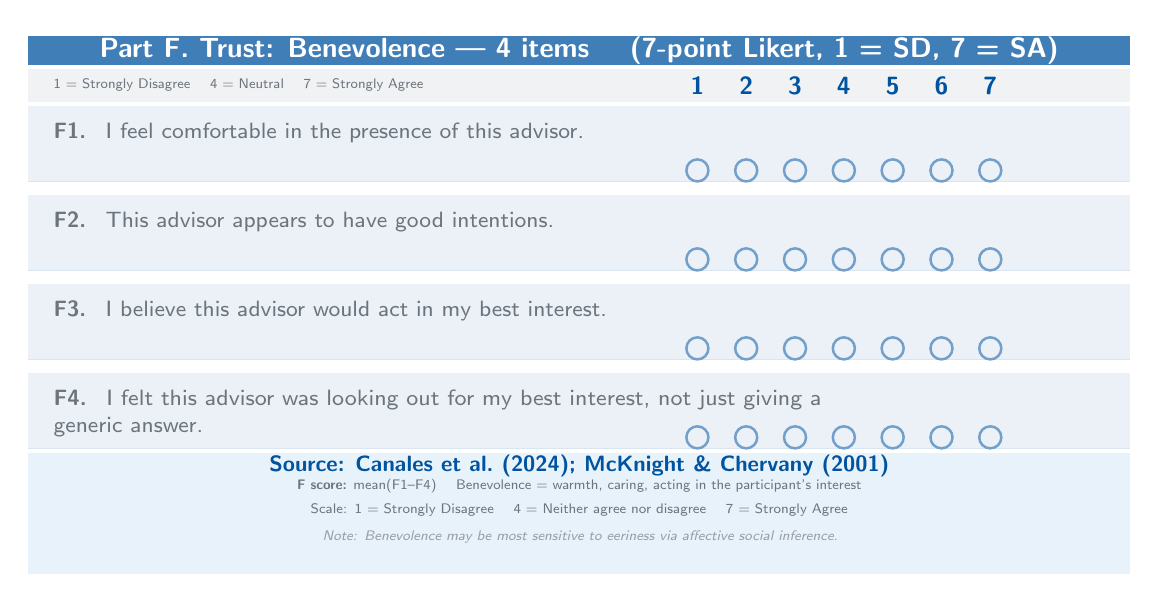
\begin{tikzpicture}[x=1cm, y=1cm]

  %% Header
  \fill[kblue!75] (0.0,6.55) rectangle (14.0,6.92);
  \node[font=\normalsize\sffamily\bfseries, text=white] at (7.0,6.73)
    {Part F. Trust: Benevolence --- 4 items \quad (7-point Likert, 1 = SD, 7 = SA)};

  %% Scale bar
  \fill[klightgray] (0.0,6.08) rectangle (14.0,6.50);
  \node[font=\tiny\sffamily\color{kgray}, anchor=west] at (0.2,6.29)
    {1 = Strongly Disagree \quad 4 = Neutral \quad 7 = Strongly Agree};
  \foreach \i/\n in {0/1,1/2,2/3,3/4,4/5,5/6,6/7}{
    \node[font=\small\sffamily\bfseries\color{kblue}] at ({8.5+\i*0.62},6.29) {\n};
  }

  %% Items
  \foreach \y/\itlabel/\txt in {
    5.55/F1/{I feel comfortable in the presence of this advisor.},
    4.42/F2/{This advisor appears to have good intentions.},
    3.29/F3/{I believe this advisor would act in my best interest.},
    2.16/F4/{I felt this advisor was looking out for my best interest, not just giving a generic answer.}
  }{
    \fill[kblue!8] (0.0,{\y-0.48}) rectangle (14.0,{\y+0.48});
    \draw[kblue!15, line width=0.3pt] (0.0,{\y-0.48}) -- (14.0,{\y-0.48});
    \node[font=\footnotesize\sffamily\color{kgray}, text width=10.2cm, anchor=north west]
      at (0.2,{\y+0.38}) {\textbf{\itlabel.} \ \txt};
    \foreach \i in {0,1,2,3,4,5,6}{
      \draw[kblue!55, line width=0.9pt] ({8.5+\i*0.62},{\y-0.34}) circle (0.14);
    }
  }

  %% Footer
  \fill[kbluelight] (0.0,0.08) rectangle (14.0,1.62);
  \node[font=\footnotesize\sffamily\bfseries\color{kblue}] at (7.0,1.46)
    {Source: Canales et al.\ (2024); McKnight \& Chervany (2001)};
  \node[font=\tiny\sffamily\color{kgray}] at (7.0,1.20)
    {\textbf{F score:} mean(F1--F4) \quad Benevolence = warmth, caring, acting in the participant's interest};
  \node[font=\tiny\sffamily\color{kgray}, text width=13cm, align=center] at (7.0,0.90)
    {Scale: 1 = Strongly Disagree \quad 4 = Neither agree nor disagree \quad 7 = Strongly Agree};
  \node[font=\tiny\sffamily\color{kgray!70}, text width=13cm, align=center] at (7.0,0.55)
    {\textit{Note: Benevolence may be most sensitive to eeriness via affective social inference.}};

\end{tikzpicture}
\end{center}
\end{frame}

%% ═══════════════════════════════════════════════════════════════════════════
%% SCENE 9 G — Part G: Trust Integrity (3 items)
%% ═══════════════════════════════════════════════════════════════════════════
\begin{frame}{Scene 9 --- Part G: Trust Integrity \textnormal{\small (Canales et al., 2024 --- 3 items, 7-point Likert)}}
\begin{center}
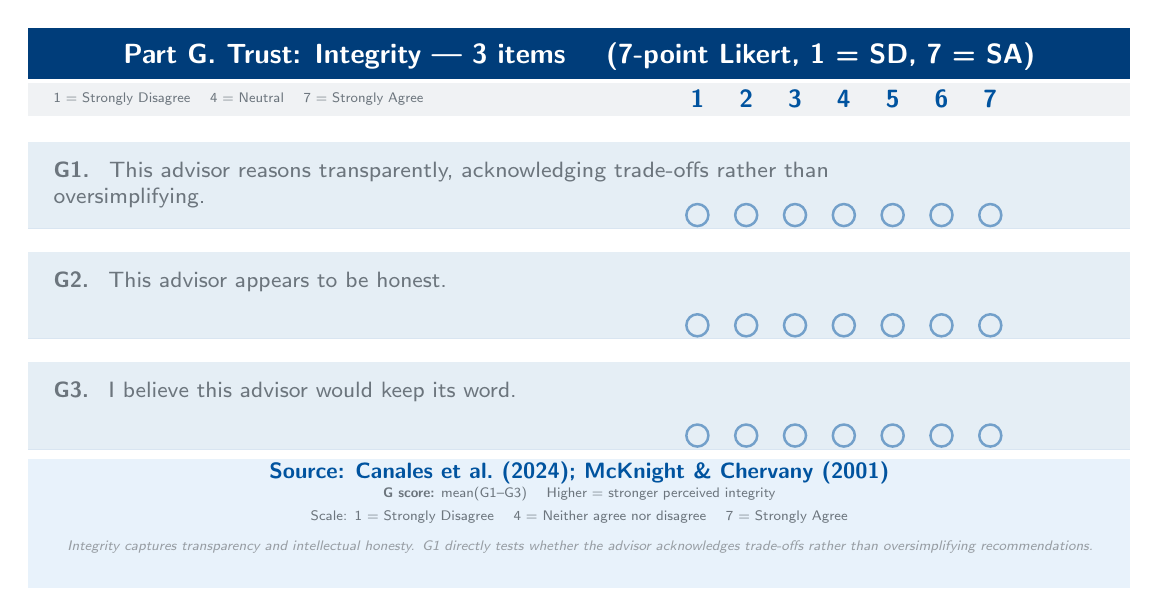
\begin{tikzpicture}[x=1cm, y=1cm]

  %% Header
  \fill[kbluedark] (0.0,6.55) rectangle (14.0,7.2);
  \node[font=\normalsize\sffamily\bfseries, text=white] at (7.0,6.83)
    {Part G. Trust: Integrity --- 3 items \quad (7-point Likert, 1 = SD, 7 = SA)};

  %% Scale bar
  \fill[klightgray] (0.0,6.08) rectangle (14.0,6.50);
  \node[font=\tiny\sffamily\color{kgray}, anchor=west] at (0.2,6.29)
    {1 = Strongly Disagree \quad 4 = Neutral \quad 7 = Strongly Agree};
  \foreach \i/\n in {0/1,1/2,2/3,3/4,4/5,5/6,6/7}{
    \node[font=\small\sffamily\bfseries\color{kblue}] at ({8.5+\i*0.62},6.29) {\n};
  }

  %% Items: 3 items at y=5.20, 3.80, 2.40, box ±0.55
  \foreach \y/\itlabel/\txt in {
    5.20/G1/{This advisor reasons transparently, acknowledging trade-offs rather than oversimplifying.},
    3.80/G2/{This advisor appears to be honest.},
    2.40/G3/{I believe this advisor would keep its word.}
  }{
    \fill[kblue!10] (0.0,{\y-0.55}) rectangle (14.0,{\y+0.55});
    \draw[kblue!15, line width=0.3pt] (0.0,{\y-0.55}) -- (14.0,{\y-0.55});
    \node[font=\footnotesize\sffamily\color{kgray}, text width=10.2cm, anchor=north west]
      at (0.2,{\y+0.42}) {\textbf{\itlabel.} \ \txt};
    \foreach \i in {0,1,2,3,4,5,6}{
      \draw[kblue!55, line width=0.9pt] ({8.5+\i*0.62},{\y-0.38}) circle (0.14);
    }
  }

  %% Footer
  \fill[kbluelight] (0.0,0.08) rectangle (14.0,1.72);
  \node[font=\footnotesize\sffamily\bfseries\color{kblue}] at (7.0,1.55)
    {Source: Canales et al.\ (2024); McKnight \& Chervany (2001)};
  \node[font=\tiny\sffamily\color{kgray}] at (7.0,1.28)
    {\textbf{G score:} mean(G1--G3) \quad Higher = stronger perceived integrity};
  \node[font=\tiny\sffamily\color{kgray}, text width=13cm, align=center] at (7.0,0.98)
    {Scale: 1 = Strongly Disagree \quad 4 = Neither agree nor disagree \quad 7 = Strongly Agree};
  \node[font=\tiny\sffamily\color{kgray!70}, text width=13cm, align=center] at (7.0,0.60)
    {\textit{Integrity captures transparency and intellectual honesty. G1 directly tests whether the advisor acknowledges trade-offs rather than oversimplifying recommendations.}};

\end{tikzpicture}
\end{center}
\end{frame}

%% ═══════════════════════════════════════════════════════════════════════════
%% SCENE 10— Part H: Recommendation Response + Attention Check
%% ═══════════════════════════════════════════════════════════════════════════
\begin{frame}{Scene 10 --- Part H: Recommendation Response + Attention Check}
\begin{center}
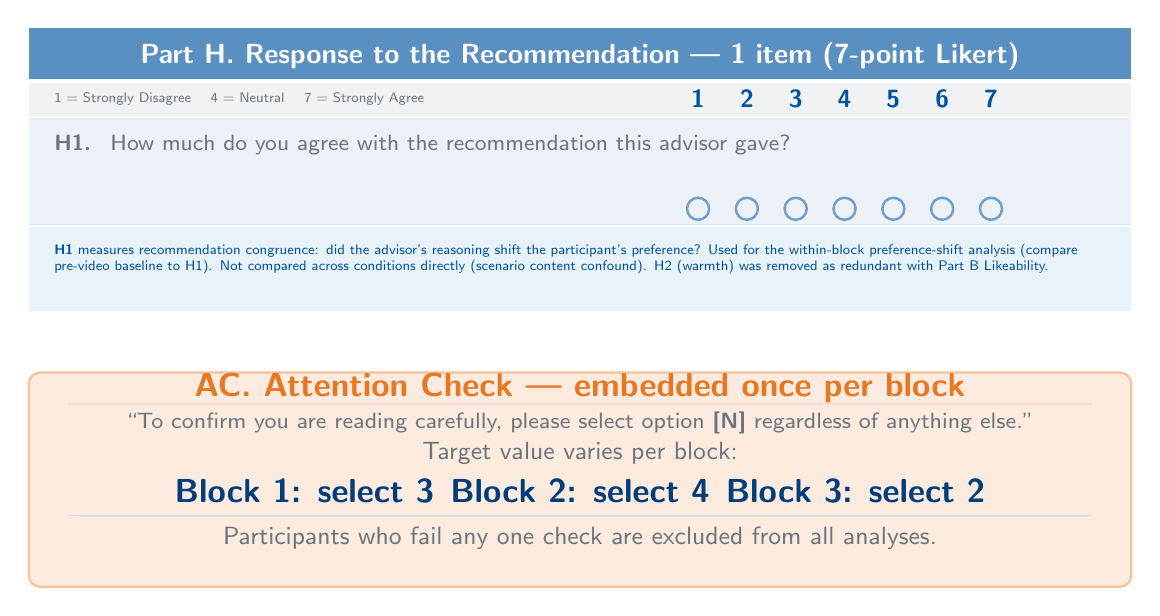
\begin{tikzpicture}[x=1cm, y=1cm]

  %% Part H header
  \fill[kblue!65] (0.0,6.55) rectangle (14.0,7.2);
  \node[font=\normalsize\sffamily\bfseries, text=white] at (7.0,6.83)
    {Part H. Response to the Recommendation --- 1 item (7-point Likert)};

  %% Scale bar
  \fill[klightgray] (0.0,6.08) rectangle (14.0,6.50);
  \node[font=\tiny\sffamily\color{kgray}, anchor=west] at (0.2,6.29)
    {1 = Strongly Disagree \quad 4 = Neutral \quad 7 = Strongly Agree};
  \foreach \i/\n in {0/1,1/2,2/3,3/4,4/5,5/6,6/7}{
    \node[font=\small\sffamily\bfseries\color{kblue}] at ({8.5+\i*0.62},6.29) {\n};
  }

  %% H1 row — taller box to accommodate 2-line text
  \fill[kblue!8] (0.0,4.70) rectangle (14.0,6.05);
  \draw[kblue!15, line width=0.3pt] (0.0,4.70) -- (14.0,4.70);
  \node[font=\footnotesize\sffamily\color{kgray}, text width=11.5cm, anchor=north west]
    at (0.2,5.96) {\textbf{H1.} \ How much do you agree with the recommendation this advisor gave?};
  \foreach \i in {0,1,2,3,4,5,6}{
    \draw[kblue!55, line width=0.9pt] ({8.5+\i*0.62},4.90) circle (0.14);
  }

  %% H note
  \fill[kbluelight] (0.0,3.60) rectangle (14.0,4.67);
  \node[font=\tiny\sffamily\color{kblue}, text width=13cm, anchor=north west] at (0.2,4.58)
    {\textbf{H1} measures recommendation congruence: did the advisor's reasoning shift the participant's preference? Used for the within-block preference-shift analysis (compare pre-video baseline to H1). Not compared across conditions directly (scenario content confound). H2 (warmth) was removed as redundant with Part B Likeability.};

  %% AC block
  \fill[korange!15, rounded corners=4pt] (0.0,0.10) rectangle (14.0,2.82);
  \draw[korange!45, rounded corners=4pt, line width=0.8pt] (0.0,0.10) rectangle (14.0,2.82);
  \node[font=\large\sffamily\bfseries\color{korange}] at (7.0,2.62)
    {AC. Attention Check --- embedded once per block};
  \draw[korange!25, line width=0.4pt] (0.5,2.42) -- (13.5,2.42);
  \node[font=\footnotesize\sffamily\color{kgray}, text width=13cm, align=center] at (7.0,2.18)
    {``To confirm you are reading carefully, please select option \textbf{[N]} regardless of anything else.''};
  \node[font=\small\sffamily\color{kgray}] at (7.0,1.80)
    {Target value varies per block:};
  \node[font=\large\sffamily\bfseries\color{kbluedark}] at (3.5,1.32)
    {Block 1: select \textbf{3}};
  \node[font=\large\sffamily\bfseries\color{kbluedark}] at (7.0,1.32)
    {Block 2: select \textbf{4}};
  \node[font=\large\sffamily\bfseries\color{kbluedark}] at (10.5,1.32)
    {Block 3: select \textbf{2}};
  \draw[kblue!20, line width=0.3pt] (0.5,1.00) -- (13.5,1.00);
  \node[font=\small\sffamily\color{kgray}] at (7.0,0.72)
    {Participants who fail any one check are excluded from all analyses.};

\end{tikzpicture}
\end{center}
\end{frame}

%% ═══════════════════════════════════════════════════════════════════════════
%% SLIDE — Scene 11: Post-Study Advisor Preference Ranking (P1)
%% ═══════════════════════════════════════════════════════════════════════════
\begin{frame}{Scene 11 --- Post-Study: Advisor Preference Ranking (P1)}
\begin{center}
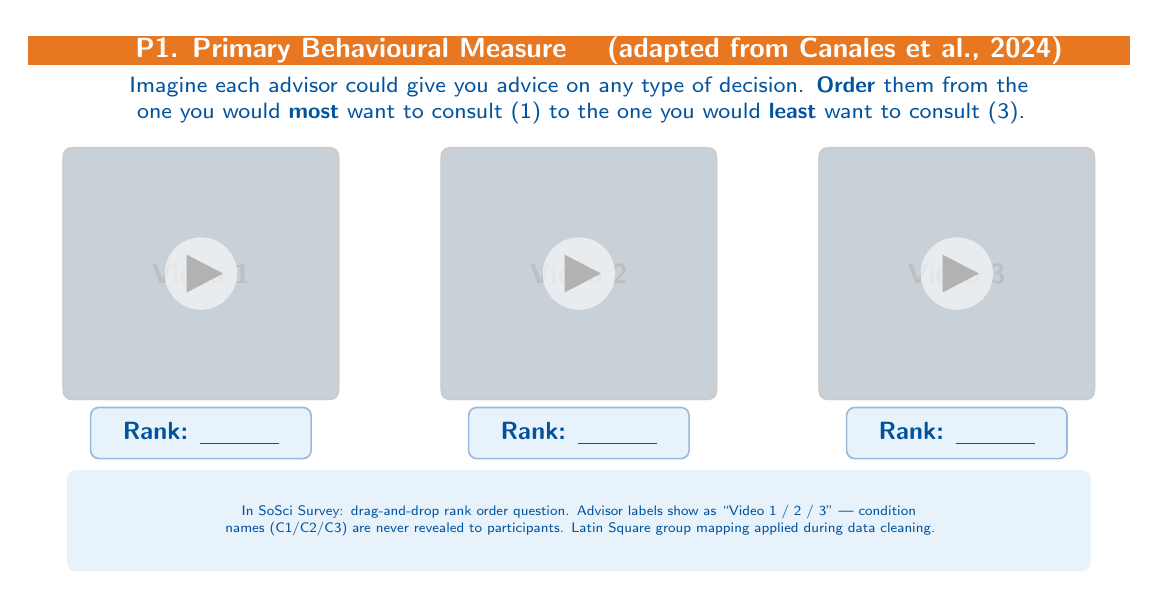
\begin{tikzpicture}[x=1cm, y=1cm]

  %% Primary measure badge
  \fill[korange] (0.0,6.55) rectangle (14.0,6.92);
  \node[font=\normalsize\sffamily\bfseries, text=white] at (7.0,6.73)
    {$\bigstar$ \quad P1. Primary Behavioural Measure \quad (adapted from Canales et al., 2024)};

  %% Question
  \node[font=\footnotesize\sffamily\color{kblue}, text width=13cm, align=center] at (7.0,6.10)
    {Imagine each advisor could give you advice on any type of decision.
     \textbf{Order} them from the one you would \textbf{most} want to consult (1) to the one you would \textbf{least} want to consult (3).};

  %% Three video boxes as nodes
  \foreach \x/\lab in {2.2/{Video 1}, 7.0/{Video 2}, 11.8/{Video 3}} {
    \fill[vidbox] ({\x-1.75},2.30) rectangle ({\x+1.75},5.50);
    \draw[gray!40, rounded corners=4pt, line width=0.5pt] ({\x-1.75},2.30) rectangle ({\x+1.75},5.50);
    \node[font=\normalsize\sffamily\bfseries\color{gray!50}] at (\x,3.90) {\lab};
    \fill[white, opacity=0.60] (\x,3.90) circle (0.46);
    \fill[gray!60] ({\x-0.18},3.66) -- ({\x-0.18},4.14) -- ({\x+0.28},3.90) -- cycle;
  }

  %% Rank slots below each box
  \foreach \x in {2.2, 7.0, 11.8} {
    \fill[kbluelight, draw=kblue!40, rounded corners=3pt, line width=0.6pt]
      ({\x-1.40},1.55) rectangle ({\x+1.40},2.20);
    \node[font=\small\sffamily\bfseries\color{kblue}] at (\x,1.87)
      {Rank: \underline{\hspace{1.0cm}}};
  }

  %% Note
  \fill[kbluelight, rounded corners=3pt] (0.5,0.12) rectangle (13.5,1.40);
  \node[font=\tiny\sffamily\color{kblue}, text width=12.5cm, align=center] at (7.0,0.76)
    {In SoSci Survey: drag-and-drop rank order question. Advisor labels show as ``Video 1 / 2 / 3'' --- condition names (C1/C2/C3) are never revealed to participants. Latin Square group mapping applied during data cleaning.};

\end{tikzpicture}
\end{center}
\end{frame}

%% ═══════════════════════════════════════════════════════════════════════════
%% PS-2 — Post-Study: P2, P3, P4 Comparative Ordering
%% ═══════════════════════════════════════════════════════════════════════════
%% ═══════════════════════════════════════════════════════════════════════════
%% PS-2 — Post-Study: P2, P3, P4 Comparative Ordering
%% ═══════════════════════════════════════════════════════════════════════════
\begin{frame}{Scene 12 --- Comparative Preference Ranking (P2, P3, P4)}
\begin{center}
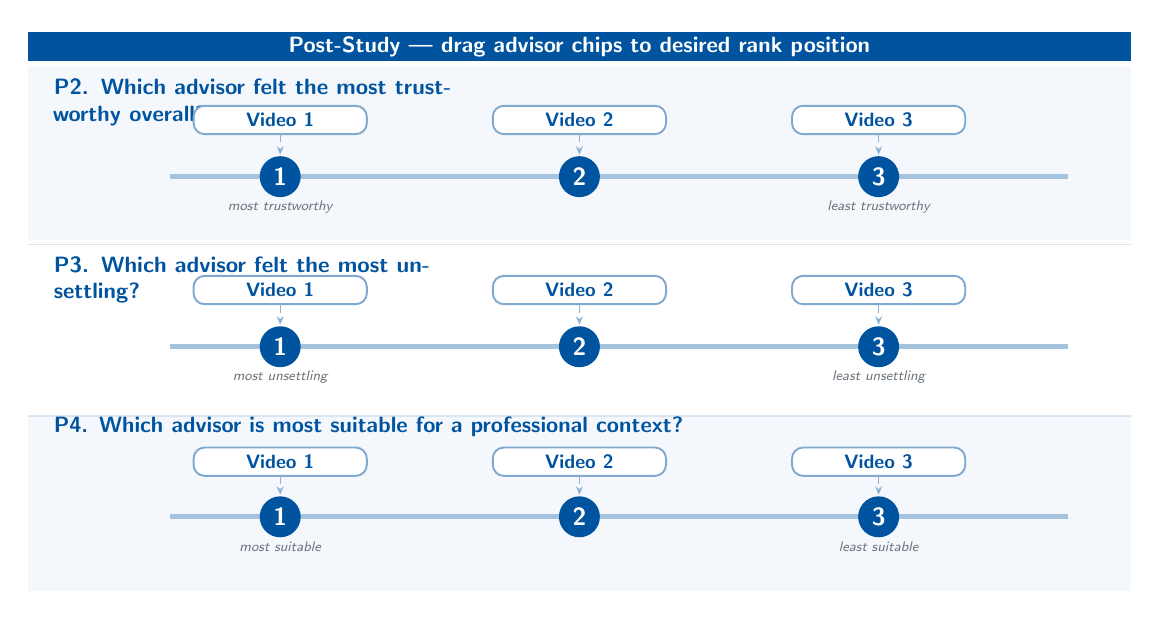
\begin{tikzpicture}[x=1cm, y=1cm]

  %% Header
  \fill[kblue] (0.0,6.55) rectangle (14.0,6.92);
  \node[font=\footnotesize\sffamily\bfseries, text=white] at (7.0,6.73)
    {Post-Study --- drag advisor chips to desired rank position};

  %% Helper macro: one rank-rail question
  %% Args: ybase, question text, anchor-left, anchor-right, fill color

  %% ── P2: Most trustworthy ──────────────────────────────────────────────
  \fill[kbluepale] (0.0,4.28) rectangle (14.0,6.48);
  \node[font=\footnotesize\sffamily\bfseries\color{kblue}, text width=5cm, anchor=north west]
    at (0.20,6.44) {P2. Which advisor felt the \textbf{most trustworthy} overall?};

  %% Rail
  \draw[kblue!35, line width=1.8pt] (1.8,5.08) -- (13.2,5.08);
  %% Snap-point circles with numbers
  \foreach \x/\n in {3.2/1, 7.0/2, 10.8/3} {
    \fill[kblue] (\x,5.08) circle (0.26);
    \node[font=\small\sffamily\bfseries, text=white] at (\x,5.08) {\n};
  }
  %% Anchor labels below circles
  \node[font=\tiny\sffamily\itshape\color{kgray}] at (3.2,4.70) {most trustworthy};
  \node[font=\tiny\sffamily\itshape\color{kgray}] at (10.8,4.70) {least trustworthy};
  %% Draggable chips above rail with dashed arrows
  \foreach \x/\lab in {3.2/{Video 1}, 7.0/{Video 2}, 10.8/{Video 3}} {
    \fill[white, rounded corners=4pt, draw=kblue!50, line width=0.7pt]
      ({\x-1.1},5.62) rectangle ({\x+1.1},5.98);
    \node[font=\scriptsize\sffamily\bfseries\color{kblue}] at (\x,5.80) {\lab};
    \draw[-{Stealth[length=3pt,width=2.5pt]}, kblue!45, dashed, line width=0.5pt]
      (\x,5.62) -- (\x,5.36);
  }

  %% ── P3: Most unsettling ───────────────────────────────────────────────
  \fill[white] (0.0,2.10) rectangle (14.0,4.22);
  \draw[kblue!15, line width=0.4pt] (0.0,4.22) -- (14.0,4.22);
  \node[font=\footnotesize\sffamily\bfseries\color{kblue}, text width=5cm, anchor=north west]
    at (0.20,4.18) {P3. Which advisor felt the \textbf{most unsettling}?};

  \draw[kblue!35, line width=1.8pt] (1.8,2.92) -- (13.2,2.92);
  \foreach \x/\n in {3.2/1, 7.0/2, 10.8/3} {
    \fill[kblue] (\x,2.92) circle (0.26);
    \node[font=\small\sffamily\bfseries, text=white] at (\x,2.92) {\n};
  }
  \node[font=\tiny\sffamily\itshape\color{kgray}] at (3.2,2.54) {most unsettling};
  \node[font=\tiny\sffamily\itshape\color{kgray}] at (10.8,2.54) {least unsettling};
  \foreach \x/\lab in {3.2/{Video 1}, 7.0/{Video 2}, 10.8/{Video 3}} {
    \fill[white, rounded corners=4pt, draw=kblue!50, line width=0.7pt]
      ({\x-1.1},3.46) rectangle ({\x+1.1},3.82);
    \node[font=\scriptsize\sffamily\bfseries\color{kblue}] at (\x,3.64) {\lab};
    \draw[-{Stealth[length=3pt,width=2.5pt]}, kblue!45, dashed, line width=0.5pt]
      (\x,3.46) -- (\x,3.20);
  }

  %% ── P4: Most suitable for professional context ────────────────────────
  \fill[kbluepale] (0.0,-0.18) rectangle (14.0,2.04);
  \draw[kblue!15, line width=0.4pt] (0.0,2.04) -- (14.0,2.04);
  \node[font=\footnotesize\sffamily\bfseries\color{kblue}, anchor=west]
    at (0.20,1.90) {P4. Which advisor is most suitable for a \textbf{professional context}?};

  \draw[kblue!35, line width=1.8pt] (1.8,0.76) -- (13.2,0.76);
  \foreach \x/\n in {3.2/1, 7.0/2, 10.8/3} {
    \fill[kblue] (\x,0.76) circle (0.26);
    \node[font=\small\sffamily\bfseries, text=white] at (\x,0.76) {\n};
  }
  \node[font=\tiny\sffamily\itshape\color{kgray}] at (3.2,0.38) {most suitable};
  \node[font=\tiny\sffamily\itshape\color{kgray}] at (10.8,0.38) {least suitable};
  \foreach \x/\lab in {3.2/{Video 1}, 7.0/{Video 2}, 10.8/{Video 3}} {
    \fill[white, rounded corners=4pt, draw=kblue!50, line width=0.7pt]
      ({\x-1.1},1.28) rectangle ({\x+1.1},1.64);
    \node[font=\scriptsize\sffamily\bfseries\color{kblue}] at (\x,1.46) {\lab};
    \draw[-{Stealth[length=3pt,width=2.5pt]}, kblue!45, dashed, line width=0.5pt]
      (\x,1.28) -- (\x,1.04);
  }

\end{tikzpicture}
\end{center}
\end{frame}

%% ═══════════════════════════════════════════════════════════════════════════
%% PS-3 — Post-Study: P5, P6, J Open Reflection
%% ═══════════════════════════════════════════════════════════════════════════
\begin{frame}{Post-Study --- Open Reflection (P5, P6, J)}
\begin{center}
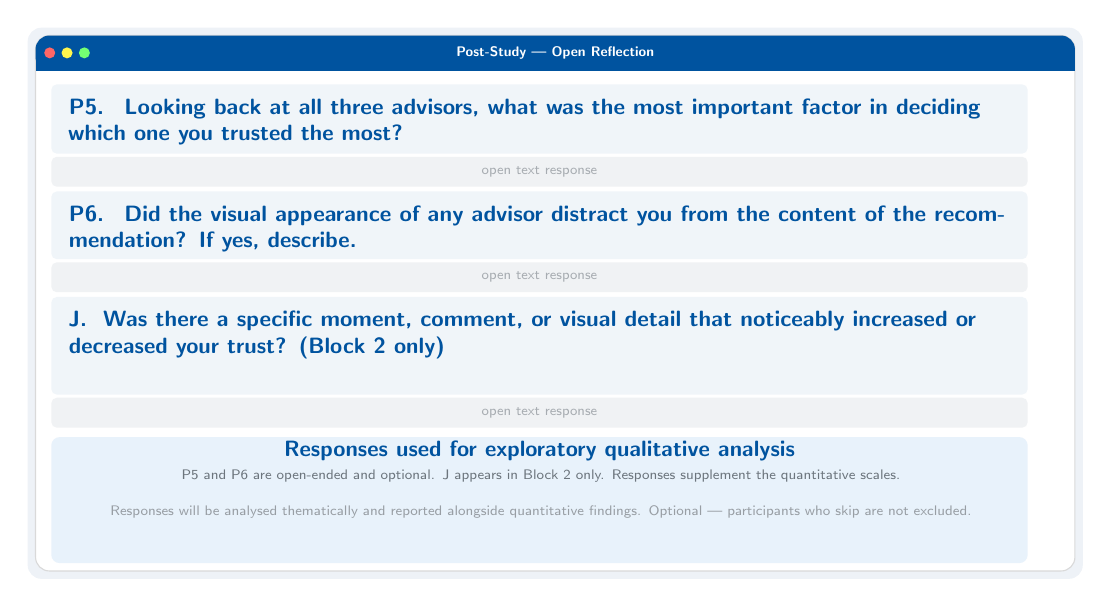
\begin{tikzpicture}[x=1cm, y=1cm]

  \browserchrome{0.4}{0.1}{13.6}{6.9}{Post-Study --- Open Reflection}
  %\progressbar{0.9}{6.4}{13.1}{0.94}{Step 8 of 9}

  %% Layout: 3 questions with generous height (0.88cm) for 2-line footnotesize text
  %% P5 blue: 5.40-6.28  P5 gray: 4.98-5.36
  %% P6 blue: 4.06-4.92  P6 gray: 3.64-4.02
  %% J  blue: 2.34-3.58  J  gray: 1.92-2.30  (taller: J may wrap to 3 lines)
  %% Note: 0.20-1.80

  %% P5
  \fill[kblue!6, rounded corners=2pt] (0.6,5.40) rectangle (13.0,6.28);
  \node[font=\footnotesize\sffamily\bfseries\color{kblue}, text width=12.0cm, anchor=north west] at (0.7,6.22)
    {P5. \ Looking back at all three advisors, what was the most important factor in deciding which one you trusted the most?};
  \fill[klightgray, rounded corners=2pt] (0.6,4.98) rectangle (13.0,5.36);
  \node[font=\tiny\sffamily\color{kgray!60}] at (6.8,5.17) {open text response};

  %% P6
  \fill[kblue!6, rounded corners=2pt] (0.6,4.06) rectangle (13.0,4.92);
  \node[font=\footnotesize\sffamily\bfseries\color{kblue}, text width=12.0cm, anchor=north west] at (0.7,4.86)
    {P6. \ Did the visual appearance of any advisor distract you from the content of the recommendation? If yes, describe.};
  \fill[klightgray, rounded corners=2pt] (0.6,3.64) rectangle (13.0,4.02);
  \node[font=\tiny\sffamily\color{kgray!60}] at (6.8,3.83) {open text response};

  %% J — taller box for potential 3-line wrap
  \fill[kblue!6, rounded corners=2pt] (0.6,2.34) rectangle (13.0,3.58);
  \node[font=\footnotesize\sffamily\bfseries\color{kblue}, text width=12.0cm, anchor=north west] at (0.7,3.52)
    {J. \ Was there a specific moment, comment, or visual detail that noticeably increased or decreased your trust? \textit{(Block 2 only)}};
  \fill[klightgray, rounded corners=2pt] (0.6,1.92) rectangle (13.0,2.30);
  \node[font=\tiny\sffamily\color{kgray!60}] at (6.8,2.11) {open text response};

  %% Note
  \fill[kbluelight, rounded corners=3pt] (0.6,0.20) rectangle (13.0,1.80);
  \node[font=\footnotesize\sffamily\bfseries\color{kblue}] at (6.8,1.62)
    {Responses used for exploratory qualitative analysis};
  \node[font=\tiny\sffamily\color{kgray}, text width=12cm, align=center] at (6.8,1.30)
    {P5 and P6 are open-ended and optional. J appears in Block 2 only. Responses supplement the quantitative scales.};
  \node[font=\tiny\sffamily\color{kgray!70}, text width=12cm, align=center] at (6.8,0.85)
    {Responses will be analysed thematically and reported alongside quantitative findings. Optional --- participants who skip are not excluded.};

\end{tikzpicture}
\end{center}
\end{frame}

%% ═══════════════════════════════════════════════════════════════════════════
%% PS-4a — Post-Study: Part I(a) Stylisation Rating (I1)
%% ═══════════════════════════════════════════════════════════════════════════
\begin{frame}{Post-Study --- Part I(a): Visual Style Check \textnormal{\small --- Stylisation Rating (I1)}}
\begin{center}
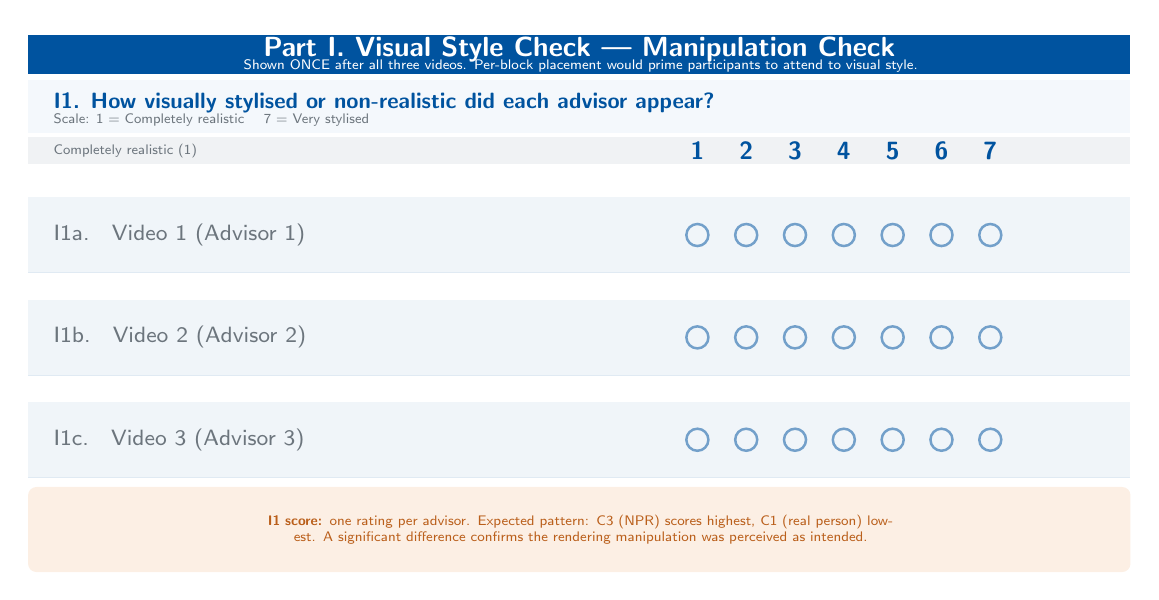
\begin{tikzpicture}[x=1cm, y=1cm]

  %% Blue header
  \fill[kblue] (0.0,6.42) rectangle (14.0,6.92);
  \node[font=\normalsize\sffamily\bfseries, text=white] at (7.0,6.74)
    {Part I. Visual Style Check --- Manipulation Check};
  \node[font=\tiny\sffamily, text=white!80, text width=13.5cm, align=center] at (7.0,6.52)
    {Shown ONCE after all three videos. Per-block placement would prime participants to attend to visual style.};

  %% I1 header
  \fill[kbluepale] (0.0,5.68) rectangle (14.0,6.35);
  \node[font=\footnotesize\sffamily\bfseries\color{kblue}, anchor=north west] at (0.2,6.31)
    {I1. How visually stylised or non-realistic did each advisor appear?};
  \node[font=\tiny\sffamily\color{kgray}, anchor=west] at (0.2,5.84)
    {Scale: 1 = Completely realistic \quad 7 = Very stylised};

  %% I1 scale bar
  \fill[klightgray] (0.0,5.28) rectangle (14.0,5.62);
  \node[font=\tiny\sffamily\color{kgray}, anchor=west] at (0.2,5.45)
    {Completely realistic (1)};
  \foreach \i/\n in {0/1,1/2,2/3,3/4,4/5,5/6,6/7}{
    \node[font=\small\sffamily\bfseries\color{kblue}] at ({8.5+\i*0.62},5.45) {\n};
  }

  %% I1a, I1b, I1c rows — spread with breathing room
  \foreach \y/\lab in {4.38/{I1a. \enspace Video 1 (Advisor 1)}, 3.08/{I1b. \enspace Video 2 (Advisor 2)}, 1.78/{I1c. \enspace Video 3 (Advisor 3)}}{
    \fill[kblue!6] (0.0,{\y-0.48}) rectangle (14.0,{\y+0.48});
    \draw[kblue!12, line width=0.3pt] (0.0,{\y-0.48}) -- (14.0,{\y-0.48});
    \node[font=\footnotesize\sffamily\color{kgray}, anchor=west] at (0.2,\y) {\lab};
    \foreach \i in {0,1,2,3,4,5,6}{
      \draw[kblue!55, line width=0.9pt] ({8.5+\i*0.62},\y) circle (0.14);
    }
  }

  %% Footer note
  \fill[korange!12, rounded corners=3pt] (0.0,0.10) rectangle (14.0,1.18);
  \node[font=\tiny\sffamily\color{korange!80!black}, text width=13.5cm, align=center] at (7.0,0.64)
    {\textbf{I1 score:} one rating per advisor. Expected pattern: C3 (NPR) scores highest, C1 (real person) lowest. A significant difference confirms the rendering manipulation was perceived as intended.};

\end{tikzpicture}
\end{center}
\end{frame}

%% ═══════════════════════════════════════════════════════════════════════════
%% PS-4b — Post-Study: Part I(b) Realism Judgement (I2)
%% ═══════════════════════════════════════════════════════════════════════════
\begin{frame}{Post-Study --- Part I(b): Visual Style Check \textnormal{\small --- Realism Judgement (I2)}}
\begin{center}
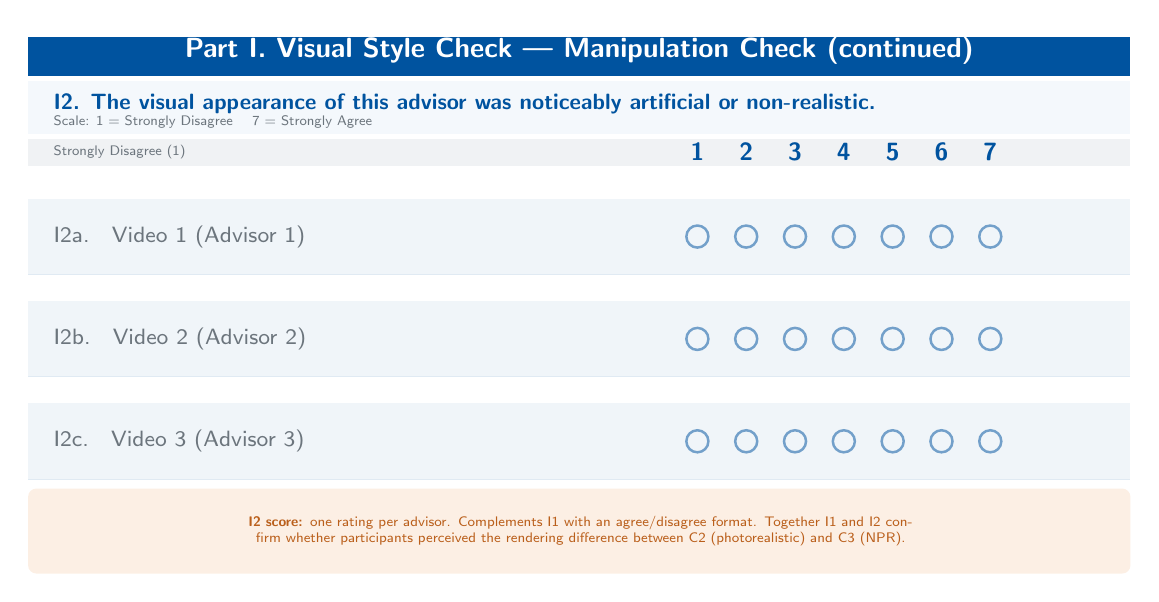
\begin{tikzpicture}[x=1cm, y=1cm]

  %% Blue header
  \fill[kblue] (0.0,6.42) rectangle (14.0,6.92);
  \node[font=\normalsize\sffamily\bfseries, text=white] at (7.0,6.74)
    {Part I. Visual Style Check --- Manipulation Check (continued)};

  %% I2 header
  \fill[kbluepale] (0.0,5.68) rectangle (14.0,6.35);
  \node[font=\footnotesize\sffamily\bfseries\color{kblue}, anchor=north west] at (0.2,6.31)
    {I2. The visual appearance of this advisor was noticeably artificial or non-realistic.};
  \node[font=\tiny\sffamily\color{kgray}, anchor=west] at (0.2,5.84)
    {Scale: 1 = Strongly Disagree \quad 7 = Strongly Agree};

  %% I2 scale bar
  \fill[klightgray] (0.0,5.28) rectangle (14.0,5.62);
  \node[font=\tiny\sffamily\color{kgray}, anchor=west] at (0.2,5.45)
    {Strongly Disagree (1)};
  \foreach \i/\n in {0/1,1/2,2/3,3/4,4/5,5/6,6/7}{
    \node[font=\small\sffamily\bfseries\color{kblue}] at ({8.5+\i*0.62},5.45) {\n};
  }

  %% I2a, I2b, I2c rows
  \foreach \y/\lab in {4.38/{I2a. \enspace Video 1 (Advisor 1)}, 3.08/{I2b. \enspace Video 2 (Advisor 2)}, 1.78/{I2c. \enspace Video 3 (Advisor 3)}}{
    \fill[kblue!6] (0.0,{\y-0.48}) rectangle (14.0,{\y+0.48});
    \draw[kblue!12, line width=0.3pt] (0.0,{\y-0.48}) -- (14.0,{\y-0.48});
    \node[font=\footnotesize\sffamily\color{kgray}, anchor=west] at (0.2,\y) {\lab};
    \foreach \i in {0,1,2,3,4,5,6}{
      \draw[kblue!55, line width=0.9pt] ({8.5+\i*0.62},\y) circle (0.14);
    }
  }

  %% Footer note
  \fill[korange!12, rounded corners=3pt] (0.0,0.10) rectangle (14.0,1.18);
  \node[font=\tiny\sffamily\color{korange!80!black}, text width=13.5cm, align=center] at (7.0,0.64)
    {\textbf{I2 score:} one rating per advisor. Complements I1 with an agree/disagree format. Together I1 and I2 confirm whether participants perceived the rendering difference between C2 (photorealistic) and C3 (NPR).};

\end{tikzpicture}
\end{center}
\end{frame}

%% ═══════════════════════════════════════════════════════════════════════════
%% PS-5a — Post-Study: Appearance Influence (HA)
%% ═══════════════════════════════════════════════════════════════════════════
\begin{frame}{Post-Study --- Appearance Influence (HA)}
\begin{center}
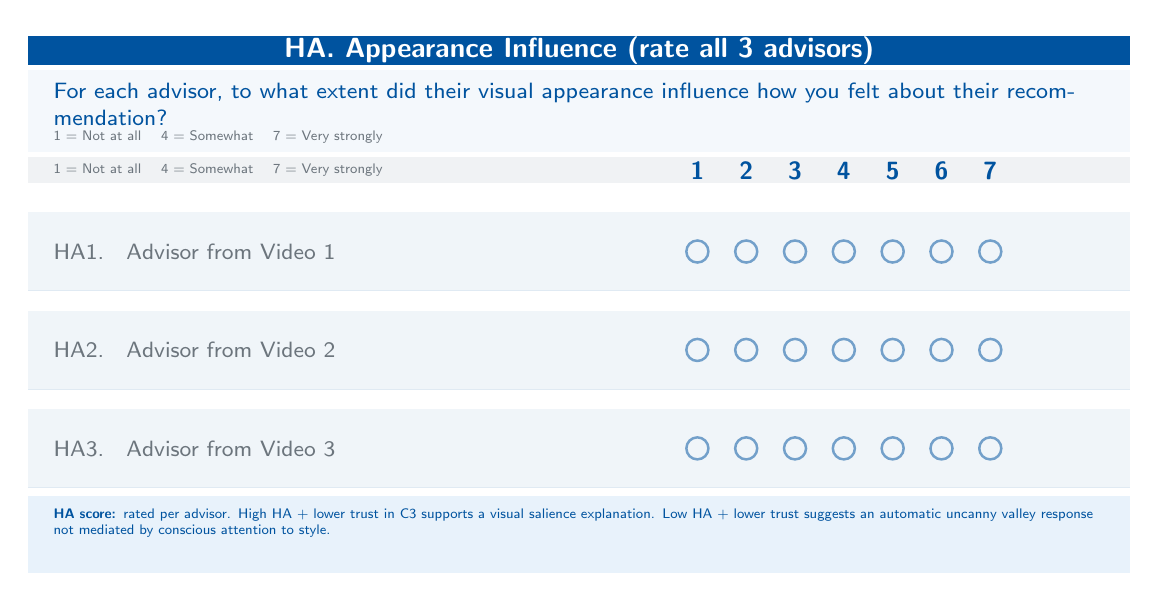
\begin{tikzpicture}[x=1cm, y=1cm]

  %% HA header
  \fill[kblue] (0.0,6.55) rectangle (14.0,6.92);
  \node[font=\normalsize\sffamily\bfseries, text=white] at (7.0,6.73)
    {HA. Appearance Influence (rate all 3 advisors)};

  %% HA question box
  \fill[kbluepale] (0.0,5.45) rectangle (14.0,6.48);
  \node[font=\footnotesize\sffamily\color{kblue}, text width=13cm, anchor=north west] at (0.2,6.44)
    {For each advisor, to what extent did their visual appearance influence how you felt about their recommendation?};
  \node[font=\tiny\sffamily\color{kgray}, anchor=west] at (0.2,5.63)
    {1 = Not at all \quad 4 = Somewhat \quad 7 = Very strongly};

  %% HA scale bar
  \fill[klightgray] (0.0,5.05) rectangle (14.0,5.38);
  \node[font=\tiny\sffamily\color{kgray}, anchor=west] at (0.2,5.21)
    {1 = Not at all \quad 4 = Somewhat \quad 7 = Very strongly};
  \foreach \i/\n in {0/1,1/2,2/3,3/4,4/5,5/6,6/7}{
    \node[font=\small\sffamily\bfseries\color{kblue}] at ({8.5+\i*0.62},5.21) {\n};
  }

  %% HA rows — spread with breathing room
  \foreach \y/\lab in {4.18/{HA1. \enspace Advisor from Video 1}, 2.93/{HA2. \enspace Advisor from Video 2}, 1.68/{HA3. \enspace Advisor from Video 3}}{
    \fill[kblue!6] (0.0,{\y-0.50}) rectangle (14.0,{\y+0.50});
    \draw[kblue!12, line width=0.3pt] (0.0,{\y-0.50}) -- (14.0,{\y-0.50});
    \node[font=\footnotesize\sffamily\color{kgray}, anchor=west] at (0.2,\y) {\lab};
    \foreach \i in {0,1,2,3,4,5,6}{
      \draw[kblue!55, line width=0.9pt] ({8.5+\i*0.62},\y) circle (0.14);
    }
  }

  %% Footer
  \fill[kbluelight] (0.0,0.10) rectangle (14.0,1.08);
  \node[font=\tiny\sffamily\color{kblue}, text width=13.2cm, anchor=north west] at (0.2,1.04)
    {\textbf{HA score:} rated per advisor. High HA + lower trust in C3 supports a visual salience explanation. Low HA + lower trust suggests an automatic uncanny valley response not mediated by conscious attention to style.};

\end{tikzpicture}
\end{center}
\end{frame}

%% ═══════════════════════════════════════════════════════════════════════════
%% SLIDE 10 — Scene 6: Debrief
%% ═══════════════════════════════════════════════════════════════════════════
\begin{frame}{Scene 13 — Debrief}
\begin{center}
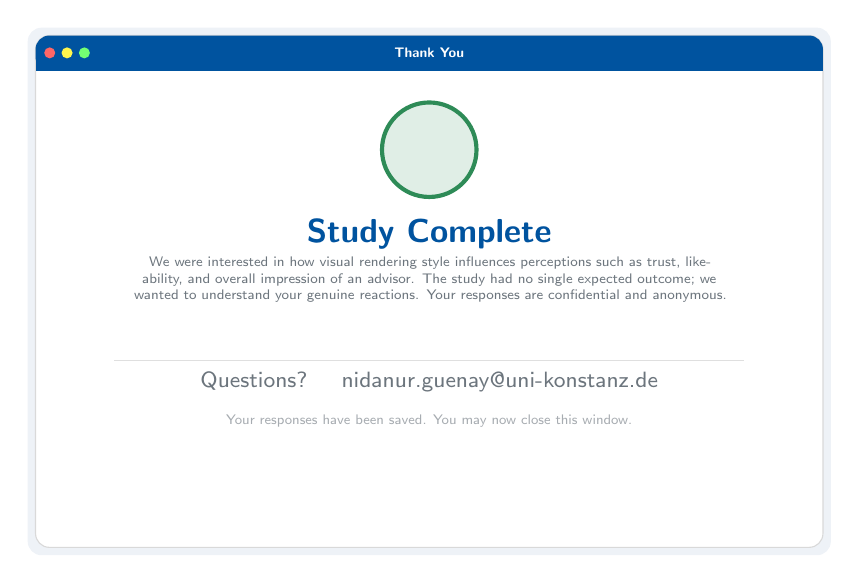
\begin{tikzpicture}[x=1cm, y=1cm]

  \browserchrome{2.0}{0.3}{12.0}{6.8}{Thank You}
  %\progressbar{2.5}{6.2}{11.5}{1.0}{Complete}

  %% Checkmark circle
  \fill[kgreen!15] (7.0,5.35) circle (0.6);
  \draw[kgreen, line width=1.5pt] (7.0,5.35) circle (0.6);
  \node[font=\large\sffamily\bfseries\color{kgreen}] at (7.0,5.35) {\checkmark};

  %% "Study Complete" at y=4.28 — clears circle bottom (4.75) by 0.22cm
  \node[font=\large\sffamily\bfseries\color{kblue}] at (7.0,4.28) {Study Complete};

  %% Body text: \tiny keeps height to ~2 lines so it does not reach "Study Complete"
  \node[font=\tiny\sffamily\color{kgray}, text width=9.0cm, align=center]
    at (7.0,3.70)
    {We were interested in how visual rendering style influences perceptions such as trust,
     likeability, and overall impression of an advisor. The study had no single expected
     outcome; we wanted to understand your genuine reactions. Your responses are
     confidential and anonymous.};

  %% Conditions strip: abbreviated single-line format to avoid wrapping
  % \fill[kbluelight, rounded corners=3pt] (2.2,2.92) rectangle (11.8,3.40);
  % \node[font=\tiny\sffamily\color{kblue}, align=center]
  %   at (7.0,3.16)
  %   {\textbf{C1:}~Real person \quad\textbullet\quad
  %    \textbf{C2:}~Avaturn realistic \quad\textbullet\quad
  %    \textbf{C3:}~Avaturn NPR stylised};

  \draw[gray!25, line width=0.3pt] (3.0,2.68) -- (11.0,2.68);

  \node[font=\footnotesize\sffamily\color{kgray}] at (7.0,2.40)
    {Questions? \quad nidanur.guenay@uni-konstanz.de};

  \node[font=\tiny\sffamily\color{kgray!60}] at (7.0,1.90)
    {Your responses have been saved. You may now close this window.};

\end{tikzpicture}
\end{center}
\end{frame}

\end{document}
